
\section{Logical View}
\label{sec_view_logical}

\subsection{Overview}

The purpose of the logical view is to specify the functional requirements of the \textit{libsafecrypto} library and describe the services that it will provide to its end-users. To this end the logical view will maintain a design model that provides a concrete description of the library's functional behaviour.

\subsection{Stakeholders}

\textbf{\textit{Developers, Maintainers, Testers}}

\textit{A description of all stakeholders is contained in Section \ref{sec:stakeholders}.}

\subsection{Top-Level Interface}

The system will provide a C API to a static or shared library that will be used to configure and operate the various cryptographic schemes. This will provide a portable library that is well supported by various processor technologies and environments. The interface will utilise the OOP principles of encapsulation (hiding the representation of a \textit{SAFEcrypto} object in order to reduce complexity) and abstraction (the definition of common interfaces to similar functional objects that are implemented differently). 

\begin{figure}[!h]
\centering
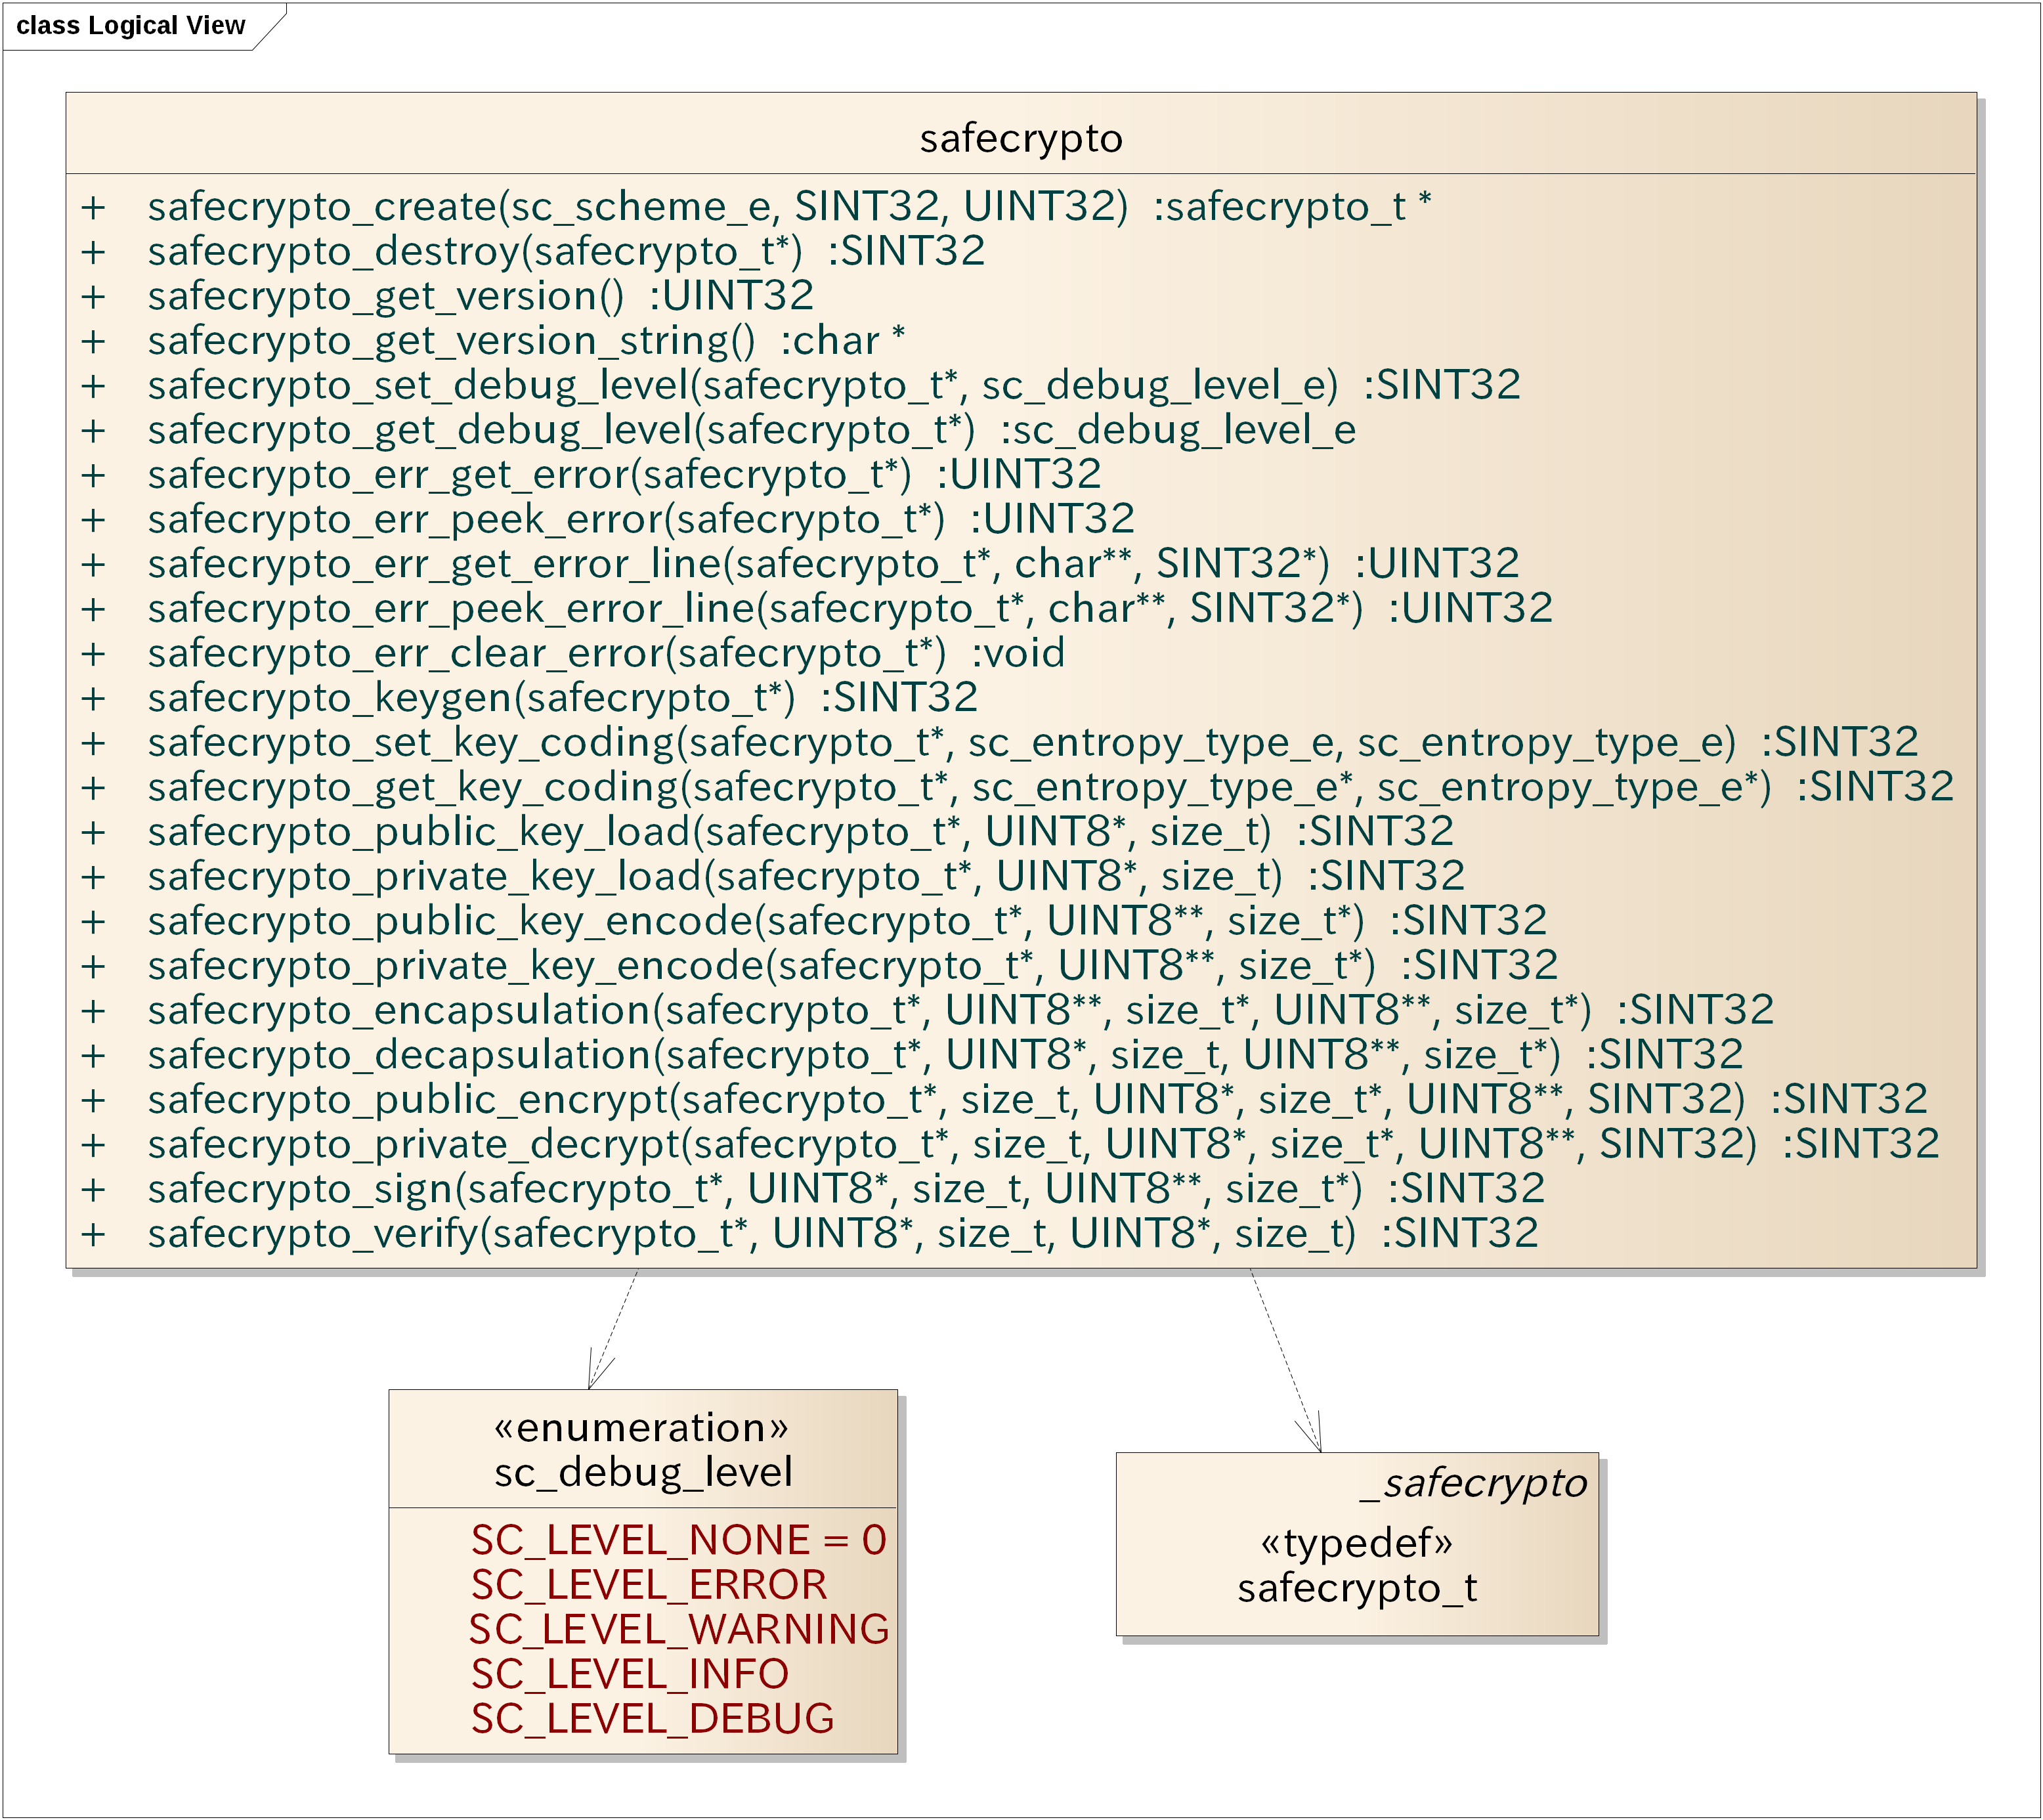
\includegraphics[width=14cm]{libsafecrypto_logical_view.png}
\caption{Class diagram of SAFEcrypto API}
\label{fig:safecrypto_api}
\end{figure}

\newpage
A description of the API is shown in Figure \ref{fig:safecrypto_api}. The principal operations of the library are to:

\begin{itemize}
\item Create/destroy an instance of a scheme with a set of parameters describing its configuration.
\item Perform cryptographic operations using an instance of the library.
\item In the event of an error, help resolve the issue by obtaining detailed information from an error queue containing human readable strings.
\end{itemize}

Each instance of the \textit{SAFEcrypto} library will operate a single cryptographic scheme. The user's choice of scheme will be defined by an enumerated type named \textit{sc\_scheme\_e} that is passed to the \textit{safecrypto\_create()} function. The top-level of the library will consist of an Interface Layer that maps the relevant functions from each scheme in the Scheme Layer to the external API.

\begin{figure}[!h]
\centering
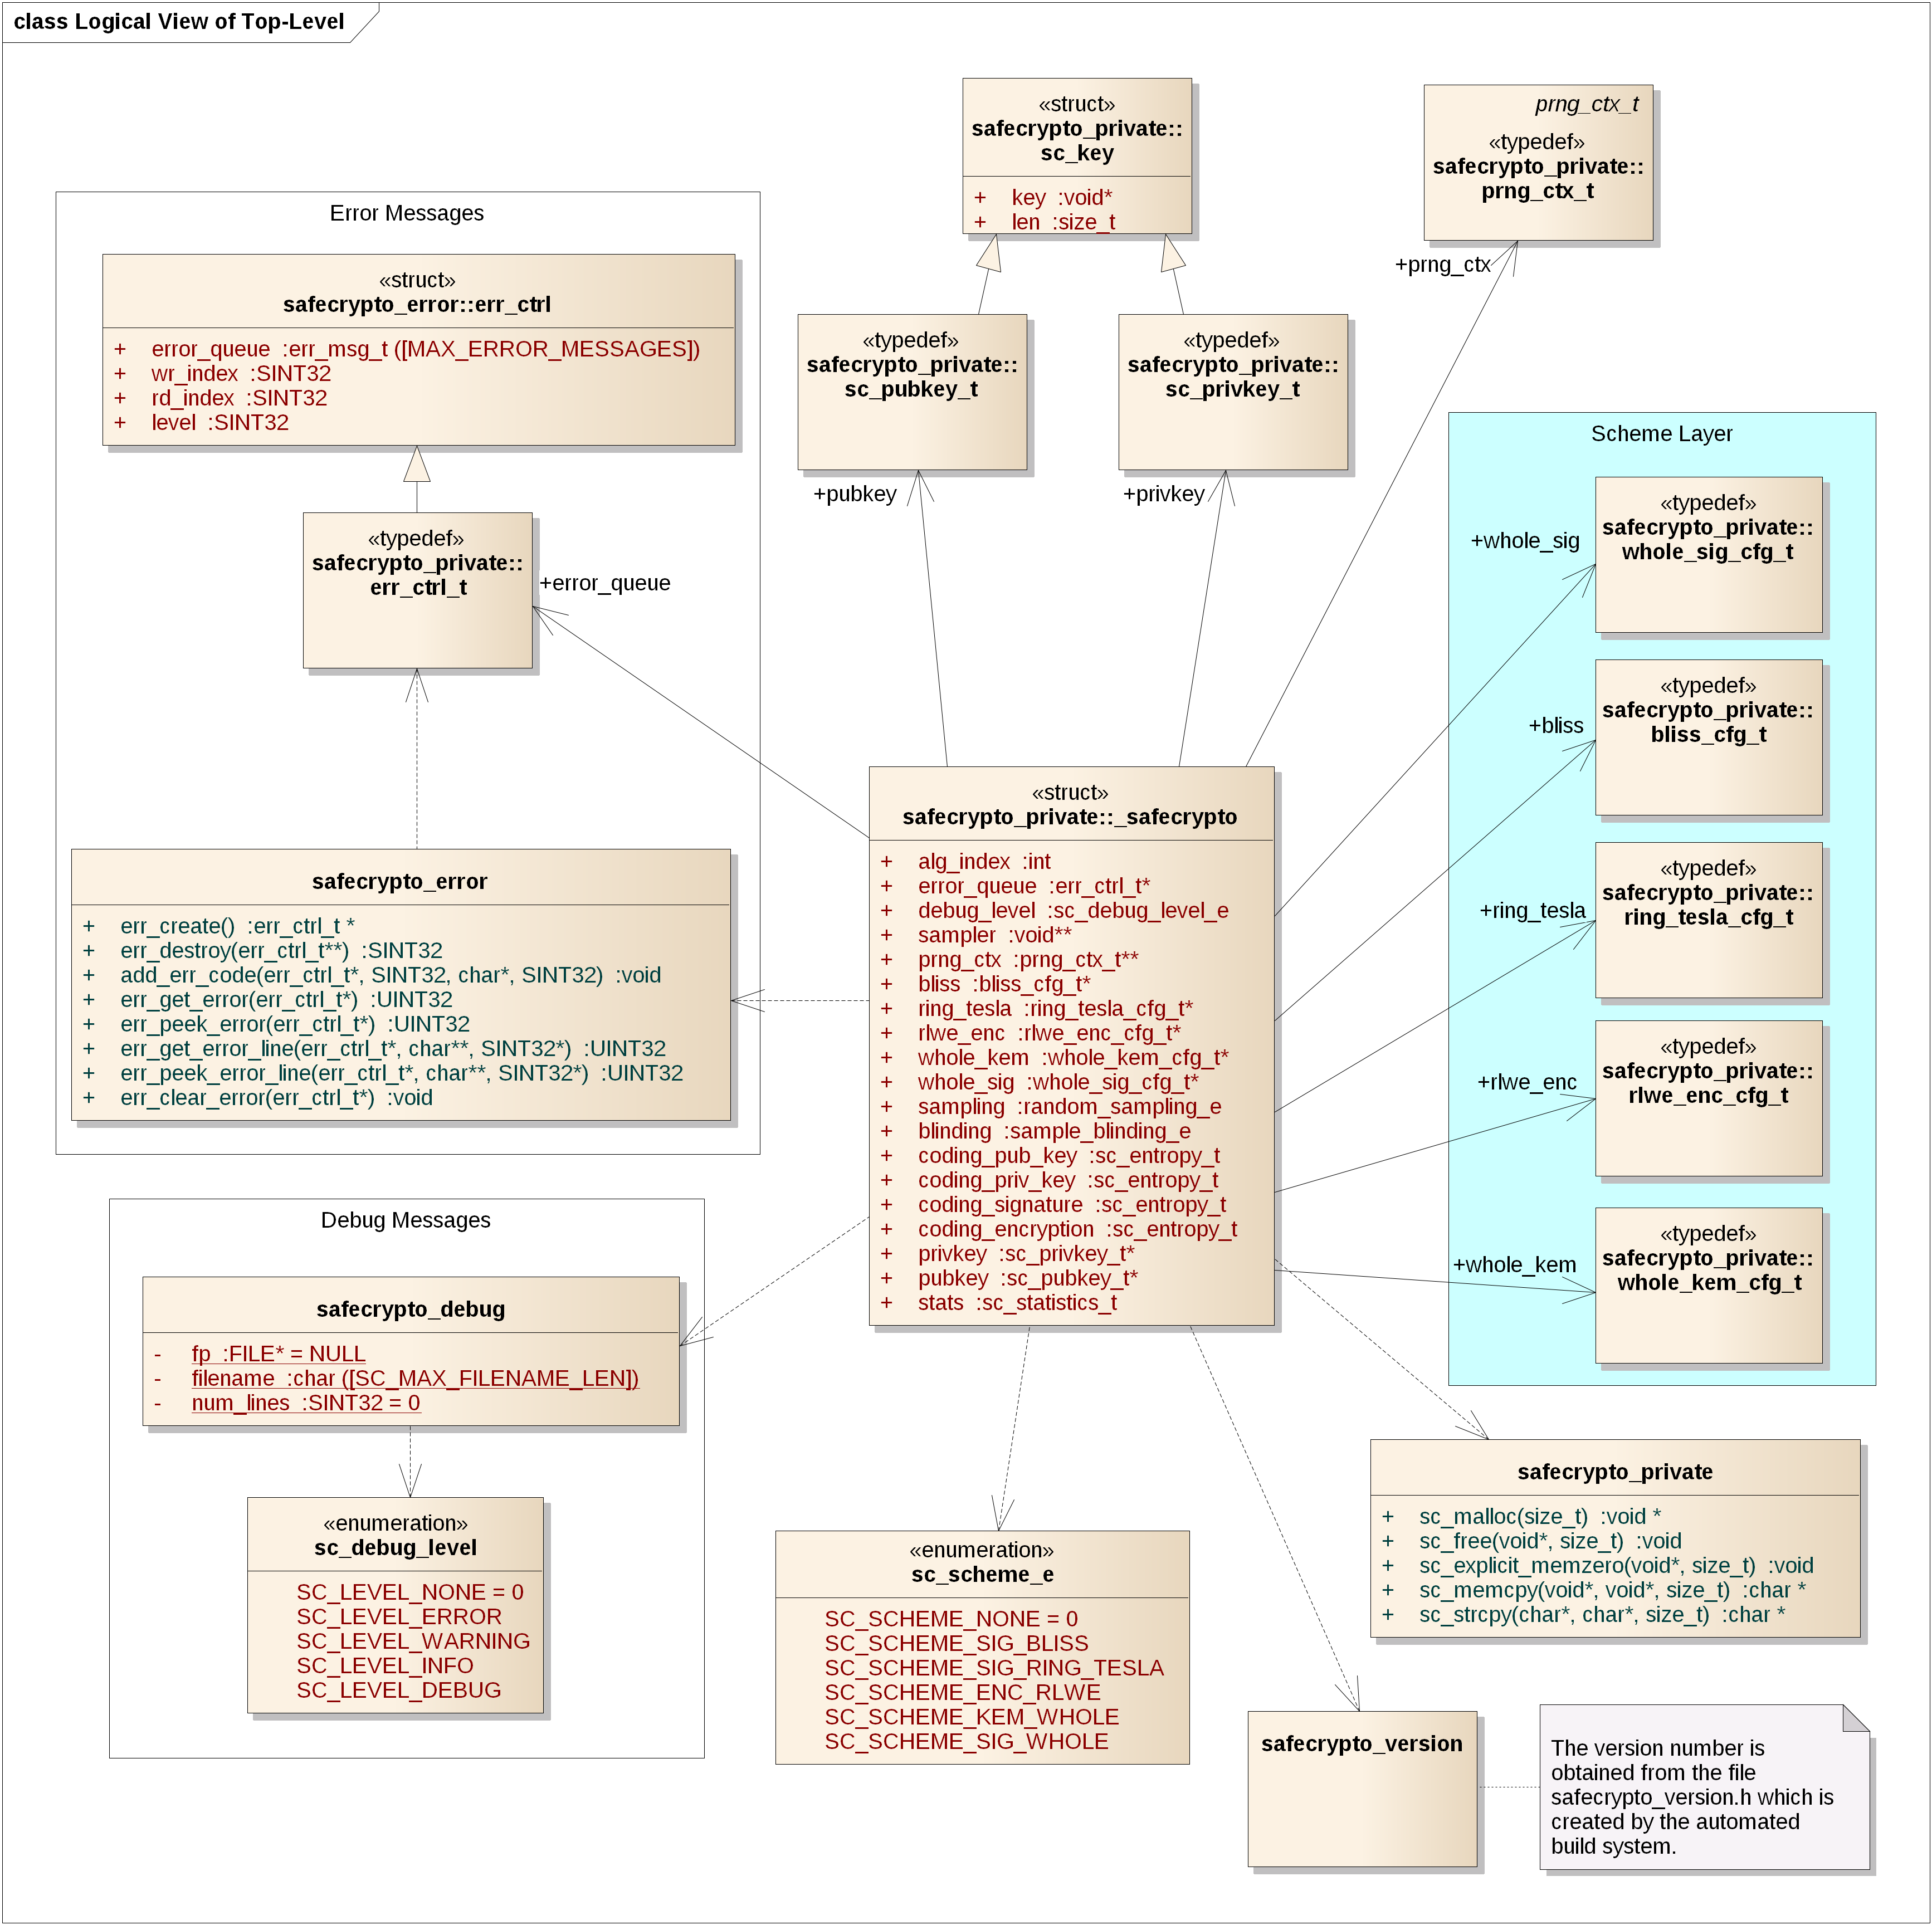
\includegraphics[width=\textwidth]{libsafecrypto_top_logical_view.png}
\caption{Class diagram of SAFEcrypto Interface Layer}
\label{fig:safecrypto_top_level}
\end{figure}

The top-level of the library is the Interface Layer which consists of an interface wrapper, as described in Figure \ref{fig:safecrypto_top_level}. This top-level will contain software subsystems for debug log printing and error queues, but is primarily used to provide access to the cryptographic schemes in the Scheme Layer. Also provided is the software version obtained from an automatically generated file named \textit{safecrypto\_version.h}.

The interface layer also provides pointers to library-wide parameters such as pointers to CSPRNG's, samplers and structures used to store key pairs.

The library will maintain a static structure that defines all cryptographic schemes and their associated functions. The function pointers utilised in this structure will encapsulate a common interface amongst all of the various schemes. This will simplify the testing and integration of the various schemes, for example (a) a range of encryption schemes can be implemented with a common test application and (b) when integrated into an application the underlying signature scheme can be arbitrarily chosen. This will permit various schemes to be implemented and evaluated using a common environment, thereby providing a fair and rapid means to evaluate various cryptographic schemes.


\newpage
\subsubsection{Error Queue}

The error queue is modelled after the OpenSSL error queue and is shown in Figure \ref{fig:safecrypto_error_queue}. The external API functions return an error code indicating success or failure only. To determine any additional information the user must interact with the error queue to obtain an error code and (optionally) the file and line number in the source code where the error occurred. The functions used to obtain the error information will pull the error from the queue, the peek functions will return the error information but will not pull the error from the queue.

\begin{figure}[!h]
\centering
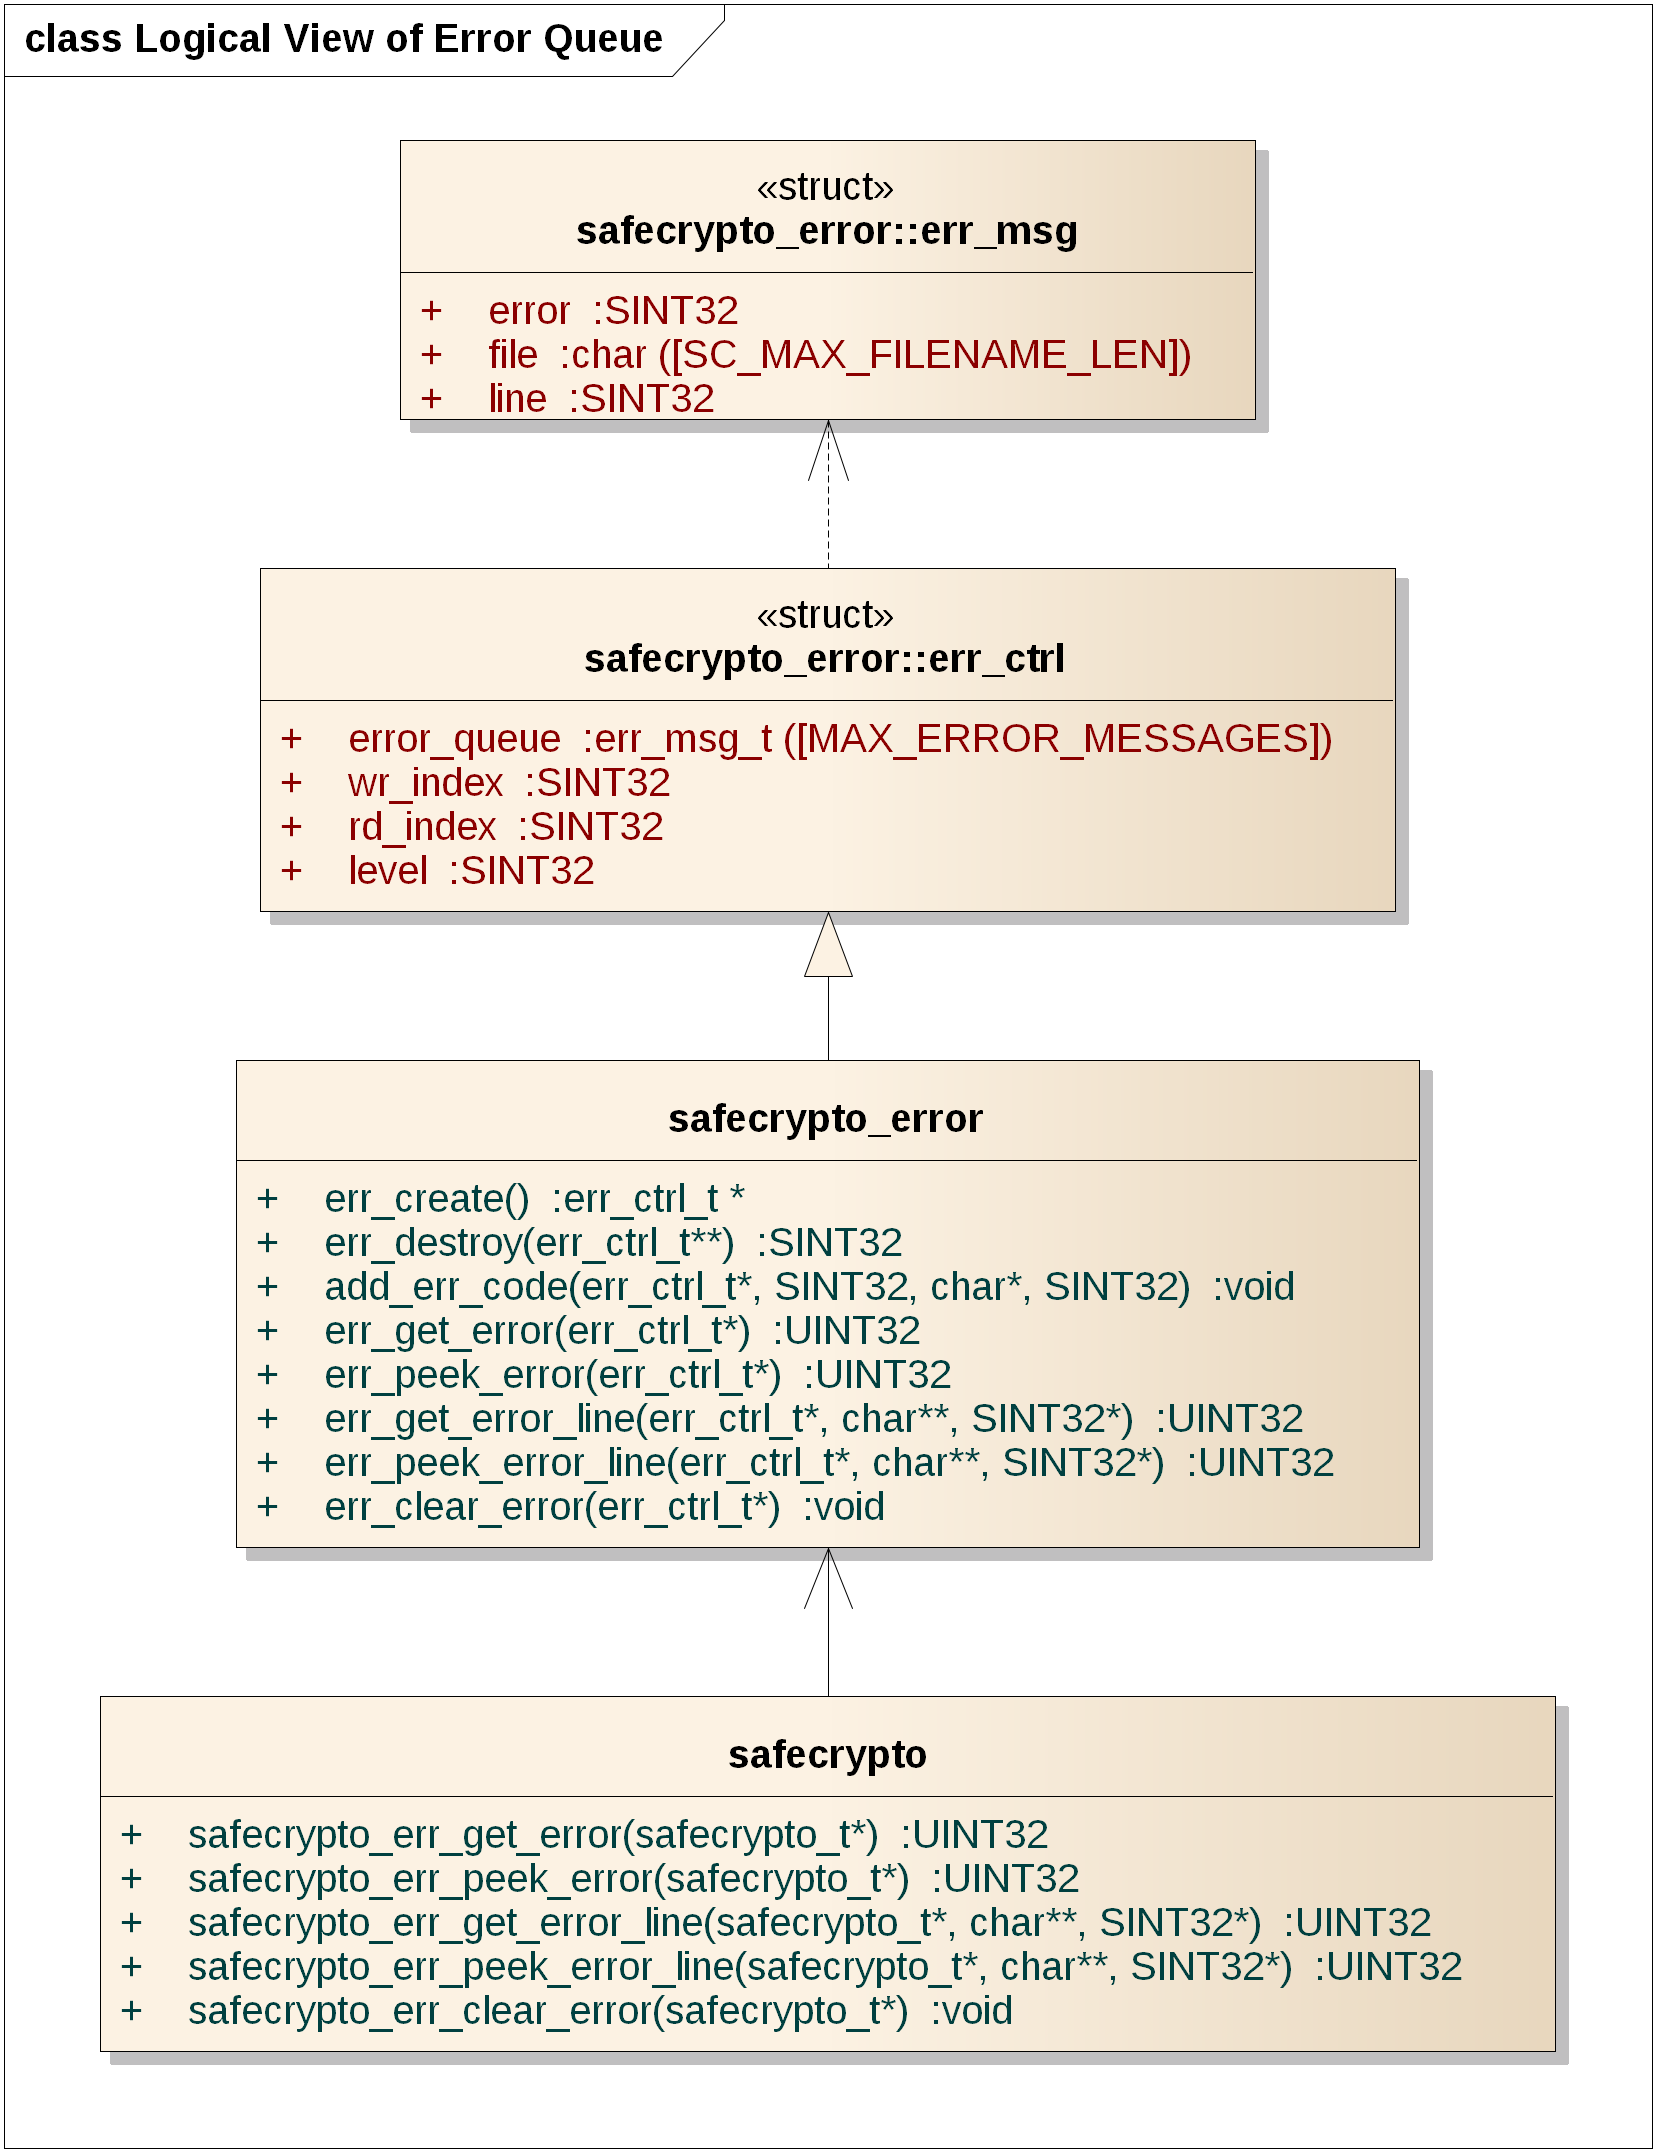
\includegraphics[width=12cm]{libsafecrypto_error_queue_logical_view.png}
\caption{Class diagram of the error queue subsystem}
\label{fig:safecrypto_error_queue}
\end{figure}


\newpage
\subsubsection{Debug Message Logging}

In order to provide a debug logging facility for developers an underlying subsystem is provided to handle all message logging to a file. \textbf{The debug logging facility is NOT to be used in any release build and will therefore be a compile-time option that is disabled by default.}

The message logging facility within the library is intended to discourage developers from utilising console print statements within their source code that could inadvertantly remain within a release build. In addition the message logging macros provide a clean and succinct means to print arrays and matrices.

The log file used to store the information will utilise a \textit{ping-pong} file store to ensure that the information logged is finite. This is achieved by recording the number of logged message lines, closing the log file when a predefined threshold is reached, renaming the file with the extension \textit{.old} and starting a new log file. This ensures that the library can run indefinately without risk of consuming the available file storage.

\begin{figure}[!h]
\centering{}
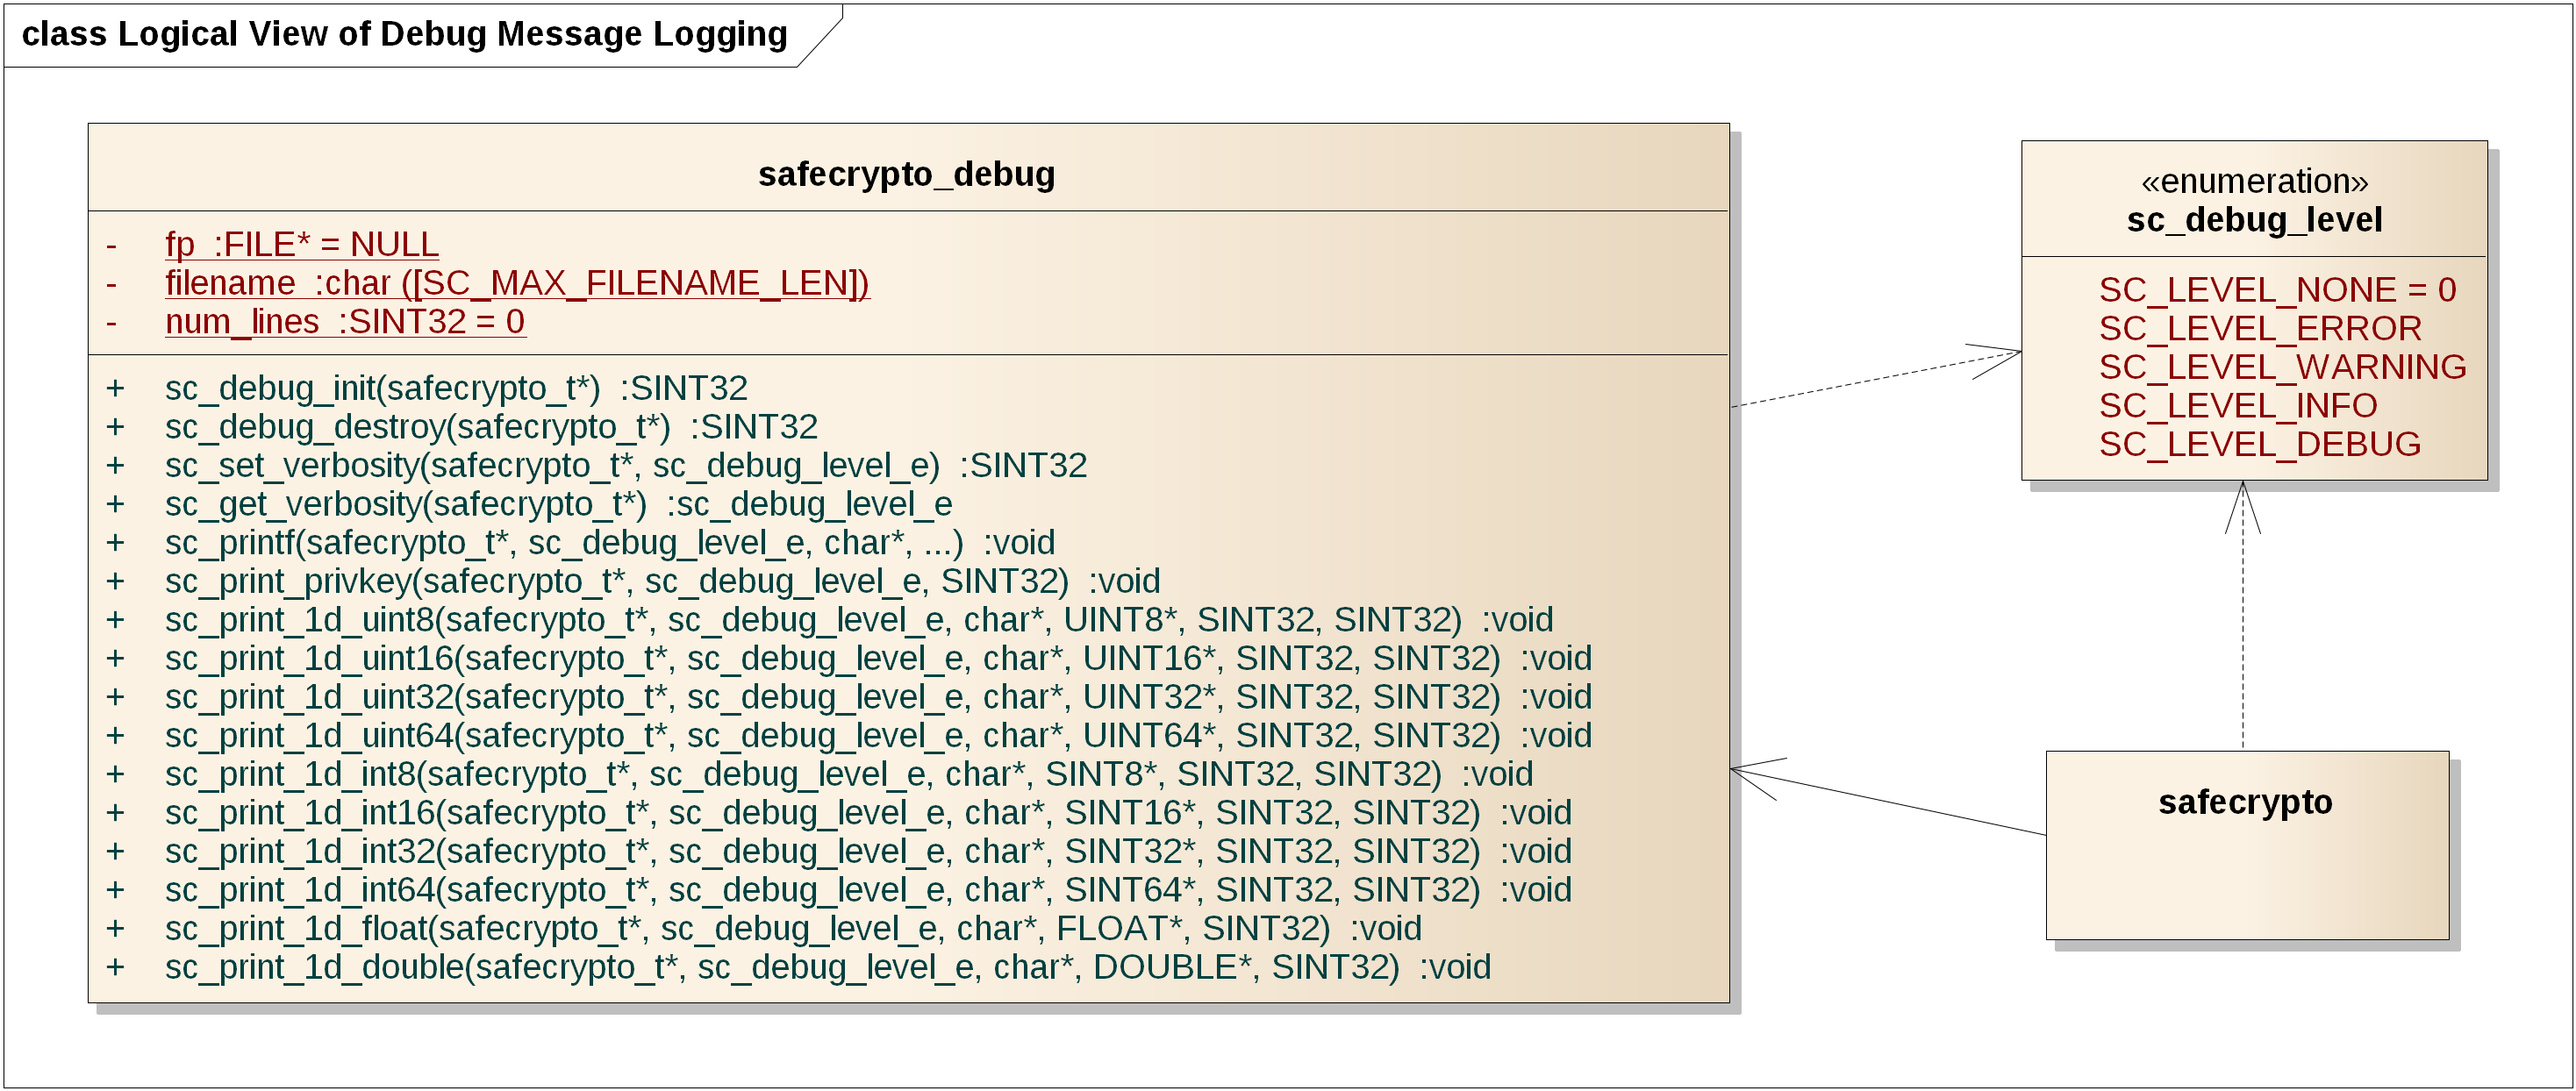
\includegraphics[width=\textwidth]{libsafecrypto_debug_logical_view.png}
\caption{Class diagram of the debug message logging subsystem}
\label{fig:safecrypto_debug_logging}
\end{figure}



\newpage
\subsection{Schemes}

The following section describes the interface to be used by all cryptographic schemes that are integrated into the \textit{SAFEcrypto} library.

\subsubsection{Creation and Destruction}

Each function call to the API must be passed a pointer to the \textit{safecrypto\_t} structure containing the instance details. The \textit{safecrypto\_create()} function is used to create all instances of the library, whilst they must be destroyed using \textit{safecrypto\_destroy()} to relinquish all memory resources. It is the responsibility of any underlying schemes to allocate memory for the public and private keys, whilst upon destruction the top-level interface must ensure that all resources including the key memory are released.

\begin{figure}[!h]
\centering
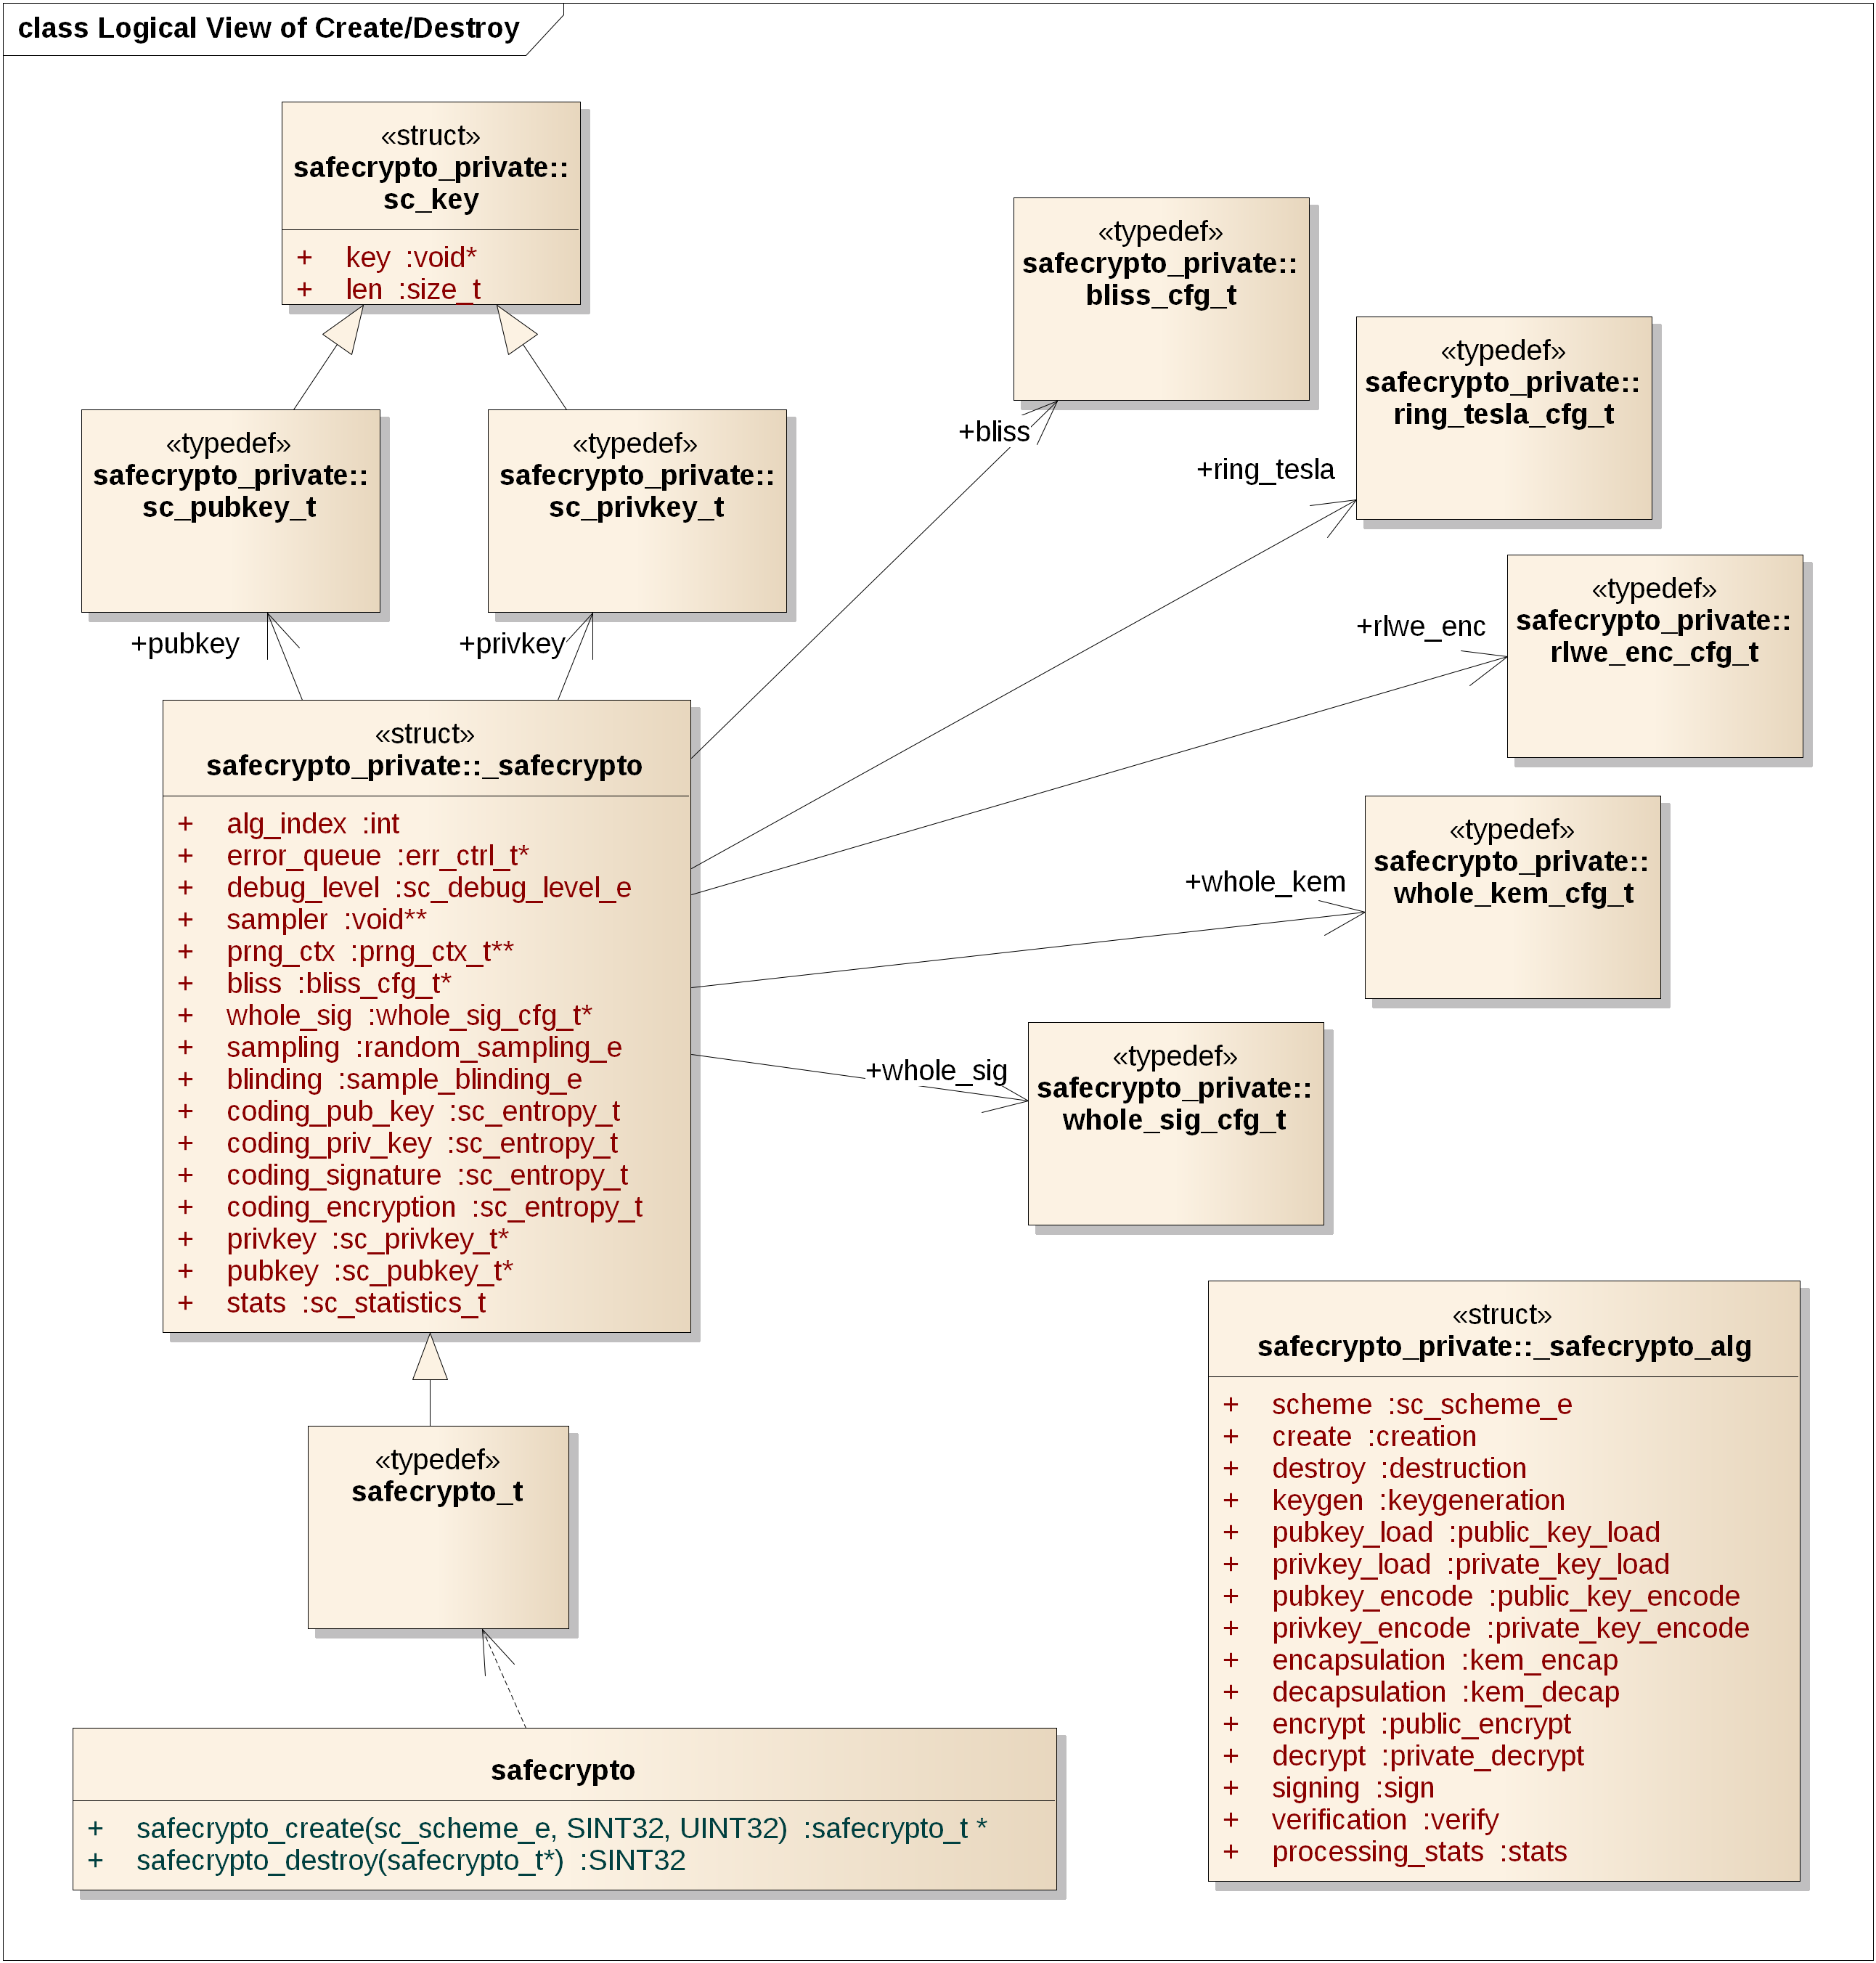
\includegraphics[width=0.9\textwidth]{libsafecrypto_create_logical_view.png}
\caption{Class diagram of the SAFEcrypto create/destroy interface}
\label{fig:safecrypto_instance}
\end{figure}


\subsubsection{Key Generation, Loading and Encoding}

All cryptographic operations must utilise the key generation function to generate a key-pair for the selected scheme. The key pair will be stored in the \textit{safecrypto\_t} structure, therefore it is erased when the destroy function is called. To maintain the key pair for future use or obtain the public key for distribution a load and encode function will be provided for both public and private keys. Each scheme must implement its own key load/encode routines, utilising the most suitable method to encode and compress the keys. These key manipulation routines are found using the function pointers in the \textit{safecrypto\_alg\_t} structure.

\begin{figure}[!h]
\centering
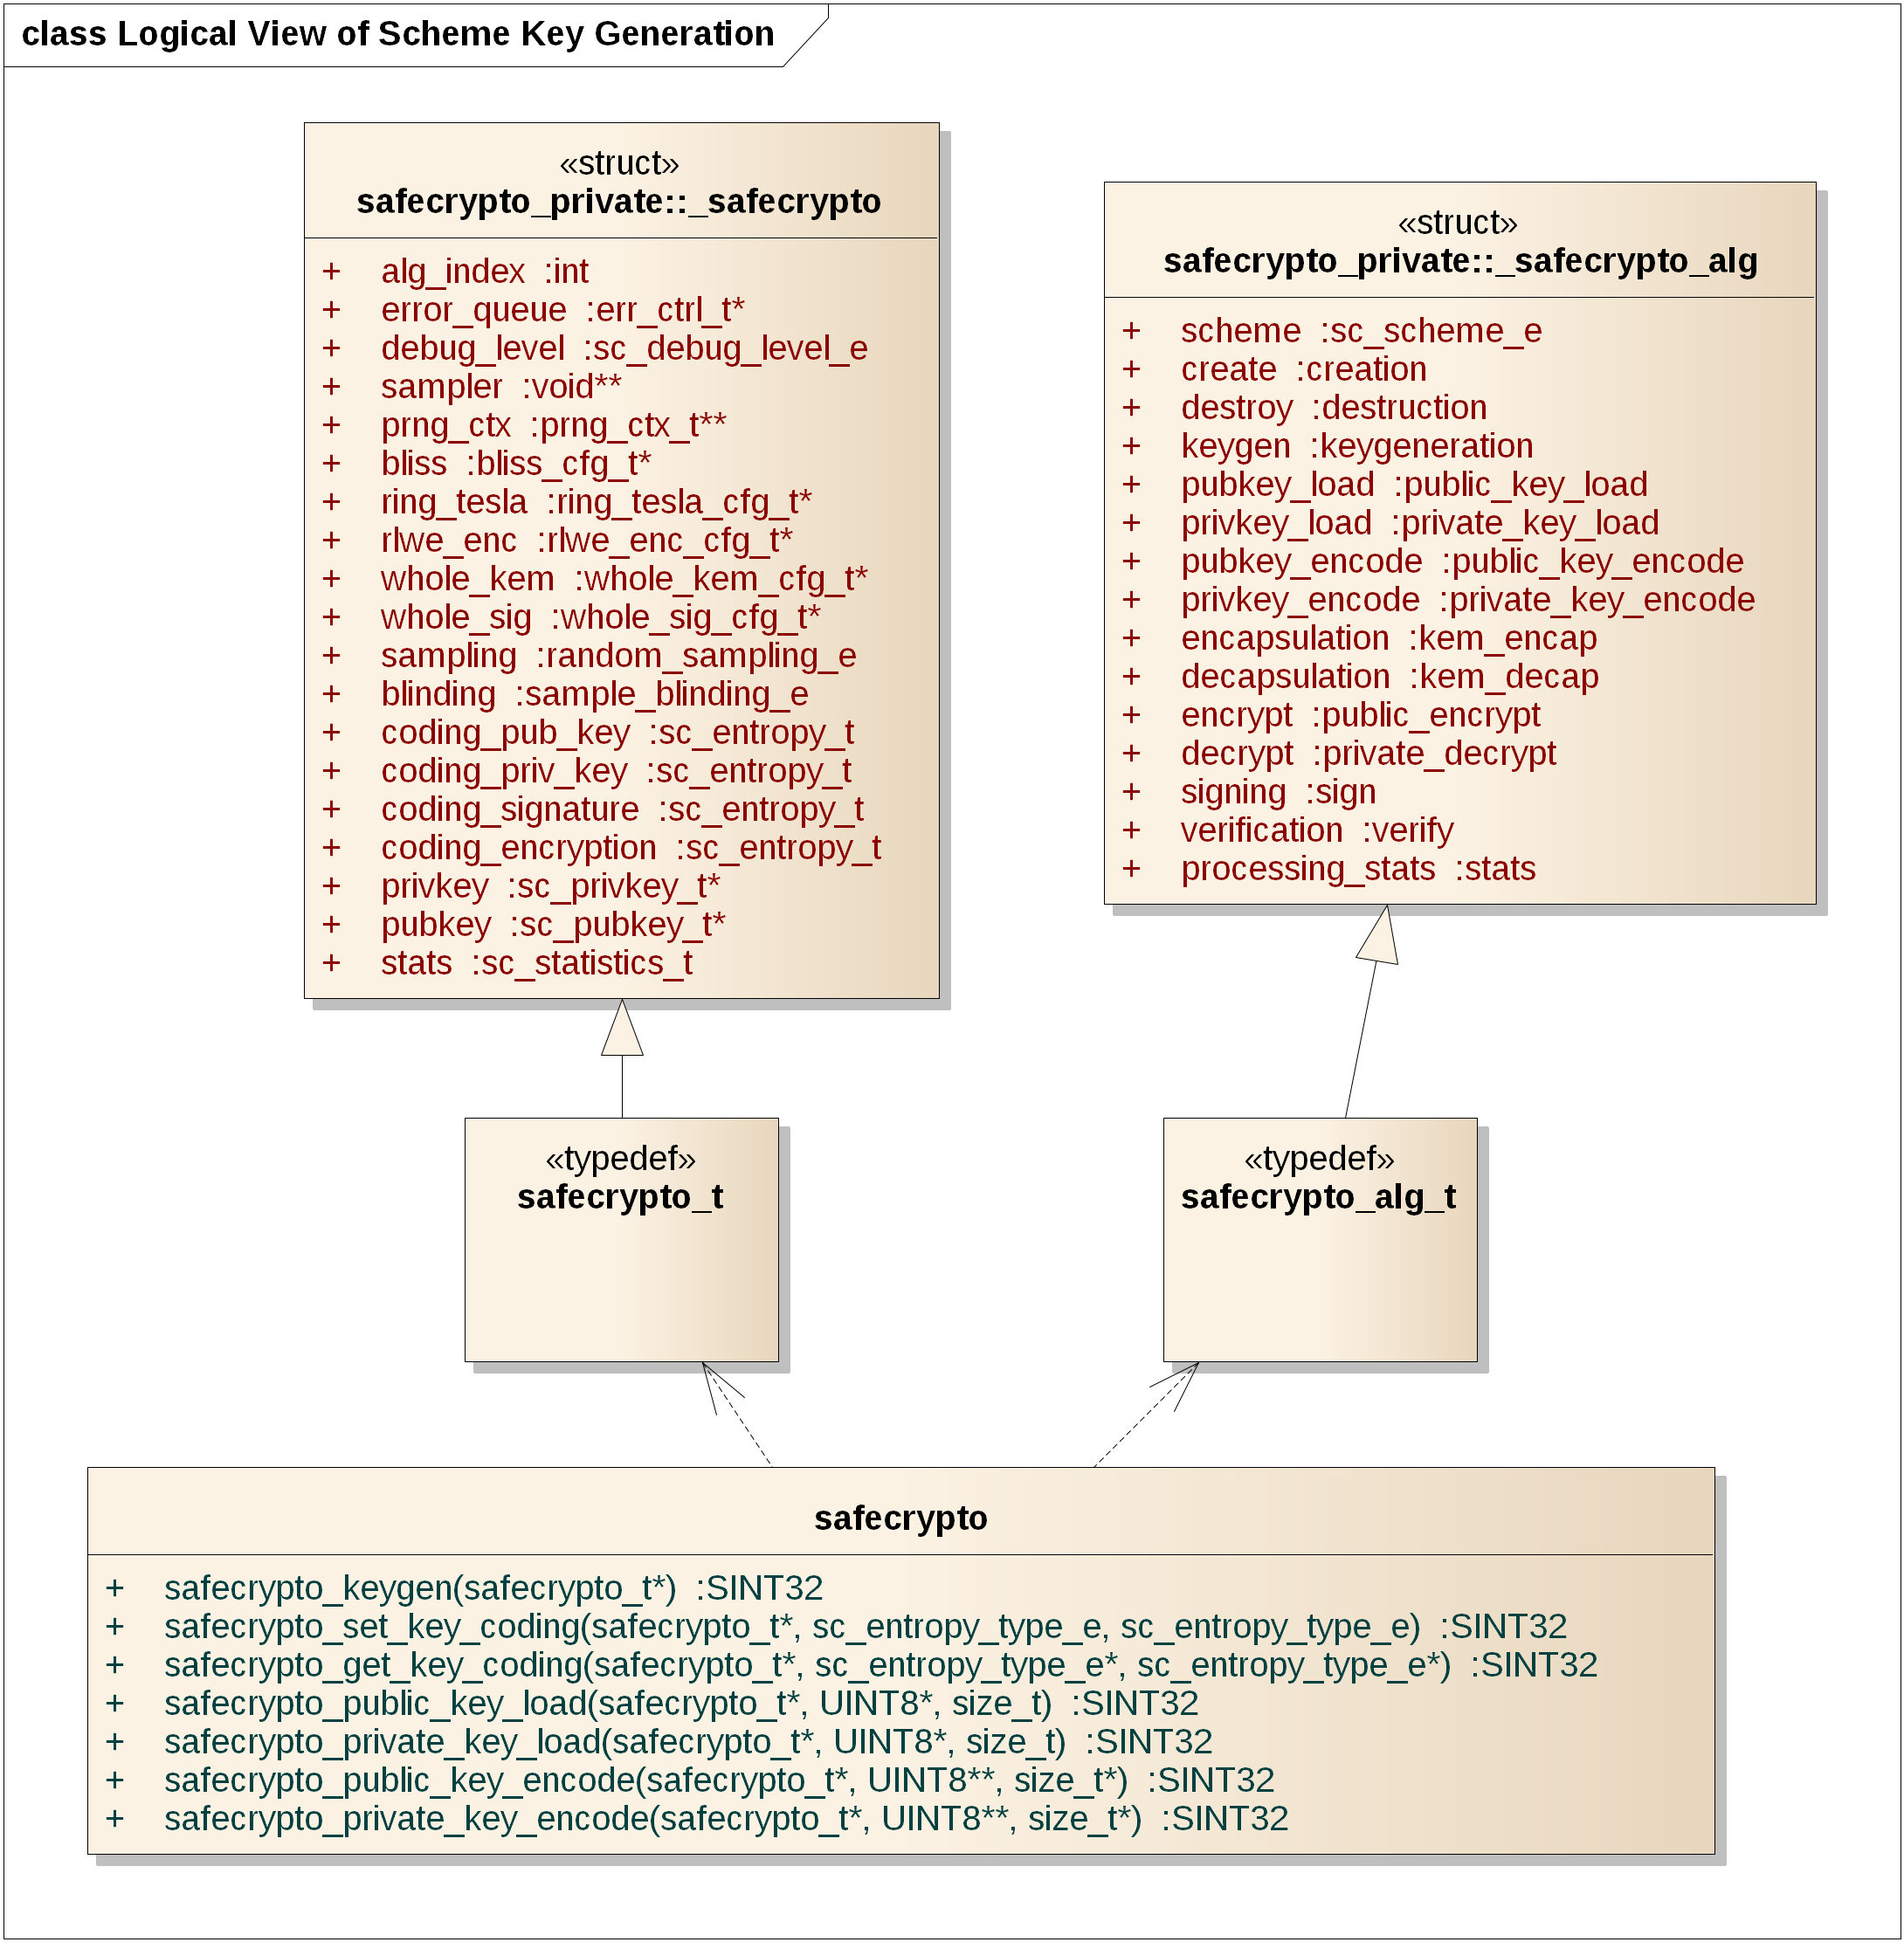
\includegraphics[width=0.9\textwidth]{libsafecrypto_keys_logical_view.png}
\caption{Class diagram of the SAFEcrypto key pair subsystem}
\label{fig:safecrypto_key_pairs}
\end{figure}


\newpage
\subsubsection{Cryptographic Operations}

A common interface will be provided for each class of scheme:

\begin{enumerate}
\item Encrypt/Decrypt
\item Encapsulate/Decapsulate
\item Sign/Verify
\item \textbf{Others to follow ...}
\end{enumerate}

All cryptographic functions will input and output arrays of data as byte streams. This will provide a generic data format that will permit cryptographic schemes to be more easily swapped as they are not restricted to a specific data structure.

\textbf{DECISION TO BE TAKEN ...}

\textit{All functions that return a byte stream will dynamically allocate memory for that byte stream on the heap, returning the number of bytes used. It is the user's responsibility to erase the contents of the byte stream when it is no longer required.}

\textbf{OR}

\textit{All functions that return a byte stream will be provided with a pointer to a buffer with a maximum length. The number of bytes used within that buffer will be returned. If more bytes are required than are available an error will be logged and a failure will be returned.}

\textbf{The first method appears to be simpler, but the cost of dynamic memory allocation cannot be overlooked. Therefore the second method is preferred in applications with high bandwidth, in particular any application where a pre-allocated queue is used to store messages and any dynamic memory allocation is a one-time setup.}


\newpage
\subsection{Utilities}

A range of utility functions will be provided as convenience libraries within the build system. These functions are intended to promote code-reuse, decrease the development time of new schemes and provide a level-playing field when comparing schemes.

\subsubsection{Arithmetic and Logical}

\begin{figure}[!h]
\centering
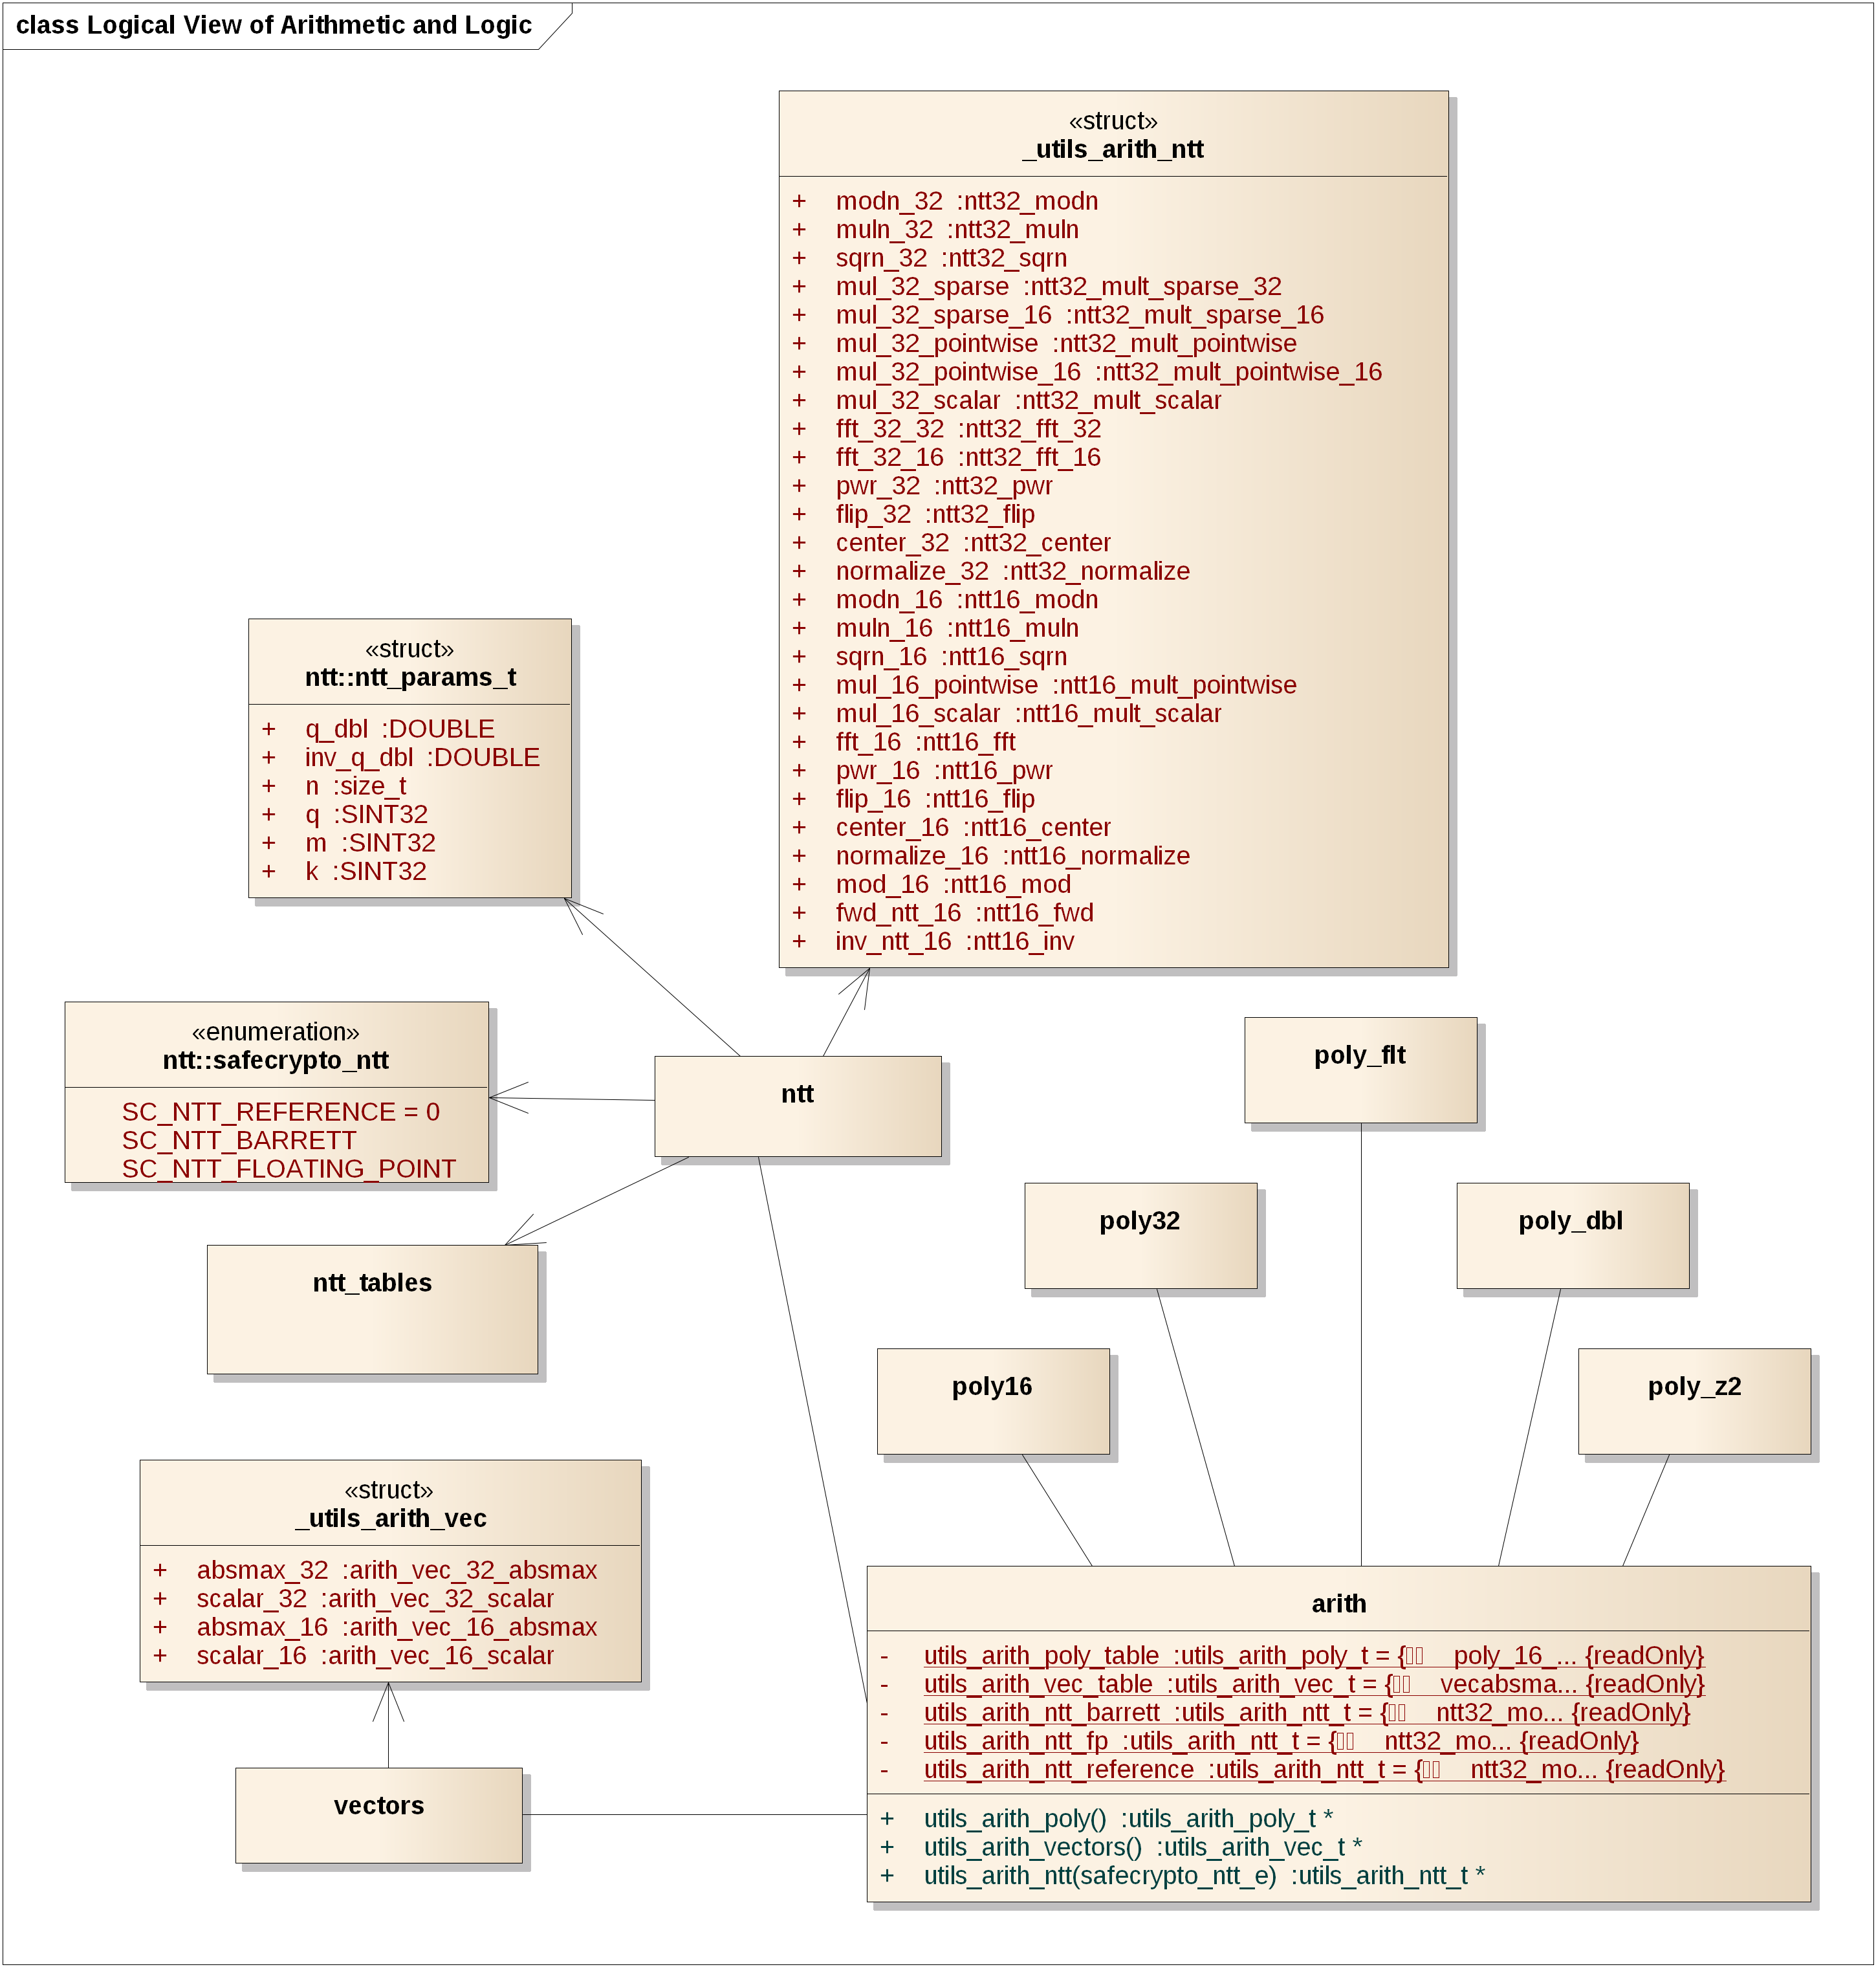
\includegraphics[width=\textwidth]{libsafecrypto_arith_logical_view.png}
\caption{Class diagram of arithmetic and logical functions}
\label{fig:safecrypto_alu}
\end{figure}

A wide range of polynomial arithmetic functions will be provided, the most compute intensive of which is the Number Theoretic Transform (NTT). Many of these functions involve finite field arithmetic and modular reduction, an operation that can be optimised with various techniques. Therefore a range of alternative methods will be provided for these functions, allowing the most suitable method to be selected depending upon the parameters of the finite field.

As shown in the class diagram of Figure \ref{fig:safecrypto_alu} the arithmetic functions are broken into two major groups, those related to the polynomial arithmetic and the NTT and those related to vector arithmetic. Additionally (and not shown in the class diagram), a range of functions and macros are provided in \textit{sc\_math.h/.c} to perform basic logical operations, primary involving endianess conversion, bit reversal, hamming weight calculations and log functions.


\subsubsection{Cryptographic}

Two types of cryptographic primitive are provided - hashing functions and CSPRNG's. Each of these primitives has a range of possible implementations that can be dynamically selected using their respective encapsulated interfaces.

In Figure \ref{fig:safecrypto_hashing} the hash functions are shown to implement a class that acts as an interface to all underlying hash algorithms. This interface class exploits a common hash interface using the functions \textit{init()}, \textit{update()} and \textit{final()}. A struct named \textit{utils\_crypto\_hash\_t} is used to maintain a state for a particular instantiation of a hash and is passed as an argument to all functions, thereby permitting multiple instances to simultaneously exist within the library.

\begin{figure}[!h]
\centering
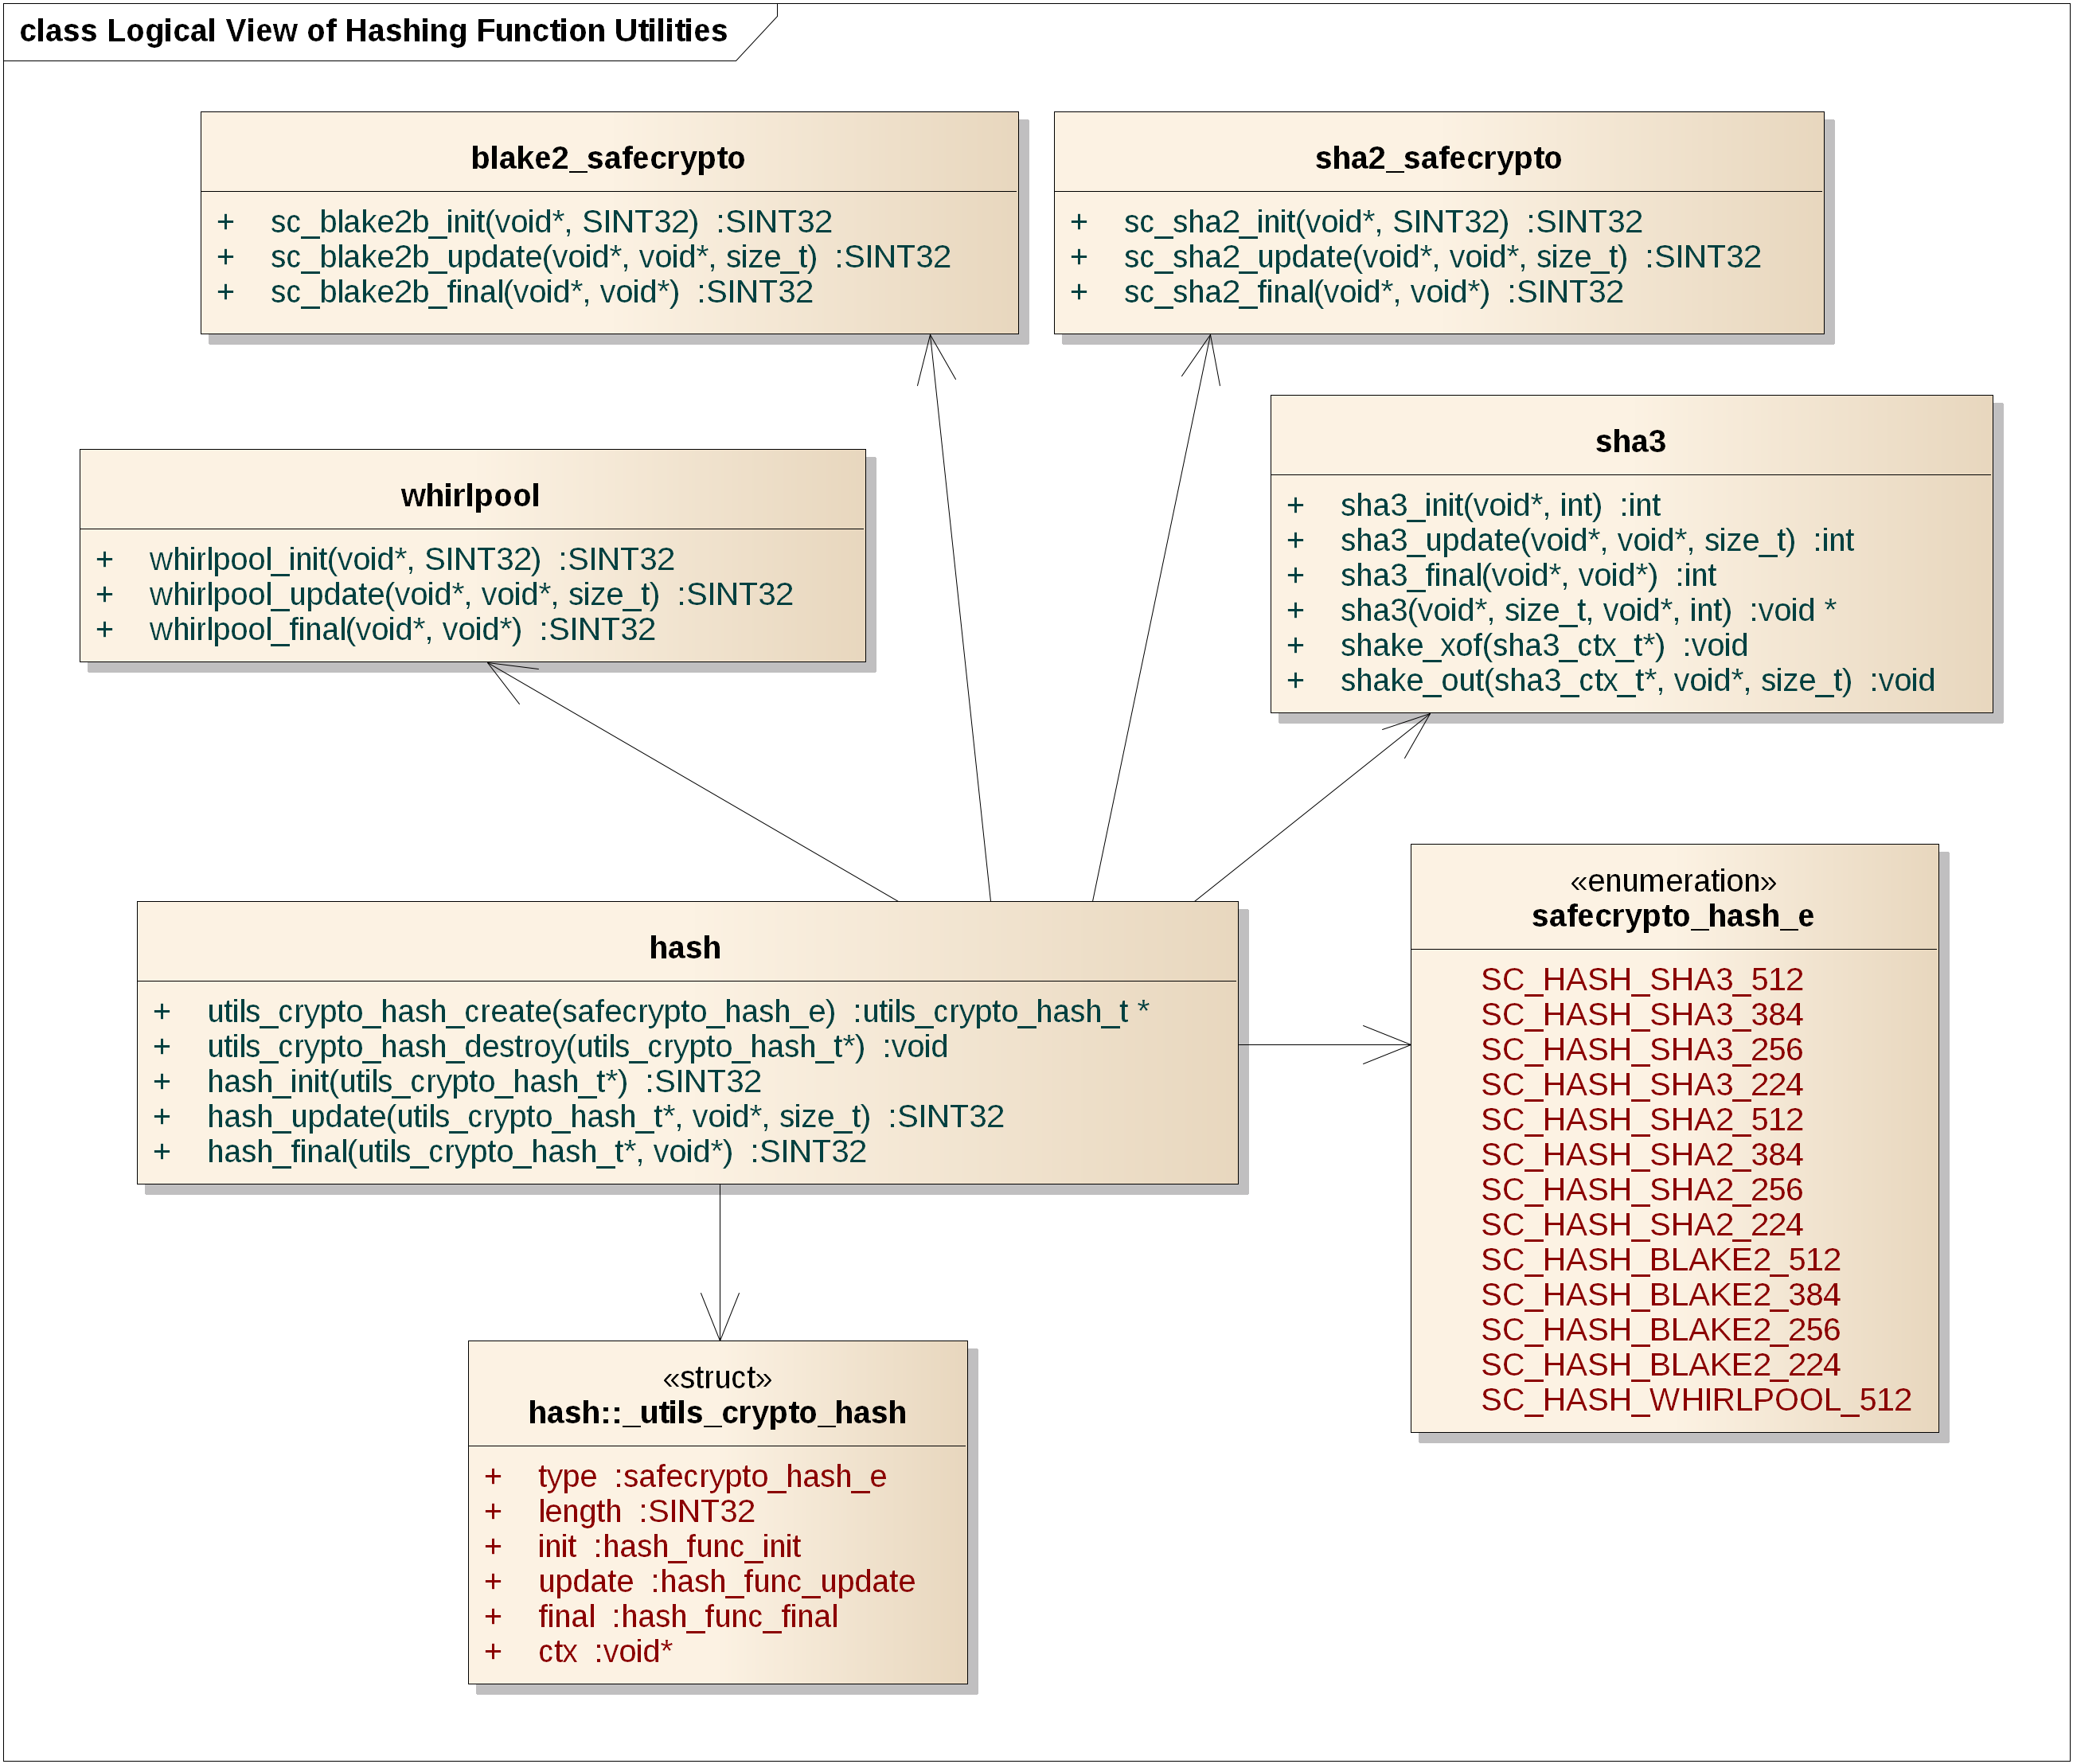
\includegraphics[width=\textwidth]{libsafecrypto_hash_logical_view.png}
\caption{Class diagram of hashing functions}
\label{fig:safecrypto_hashing}
\end{figure}

In Figure \ref{fig:safecrypto_csprng} the various CSPRNG schemes are shown to be associated with a \textit{prng} class that acts as an interface. One of a range of random number generators can be selected during instantiation of the \textit{SAFEcrypto} library, which causes a range of function pointers in the \textit{prng\_ctx\_t} struct to be set to the relevant CSPRNG scheme. This struct is then maintained to ensure that the state of the selected CSPRNG is maintained. When the user calls any of the \textit{prng} interface functions the relevant function pointer to the selected PRNG scheme is called.

\begin{figure}[!h]
\centering
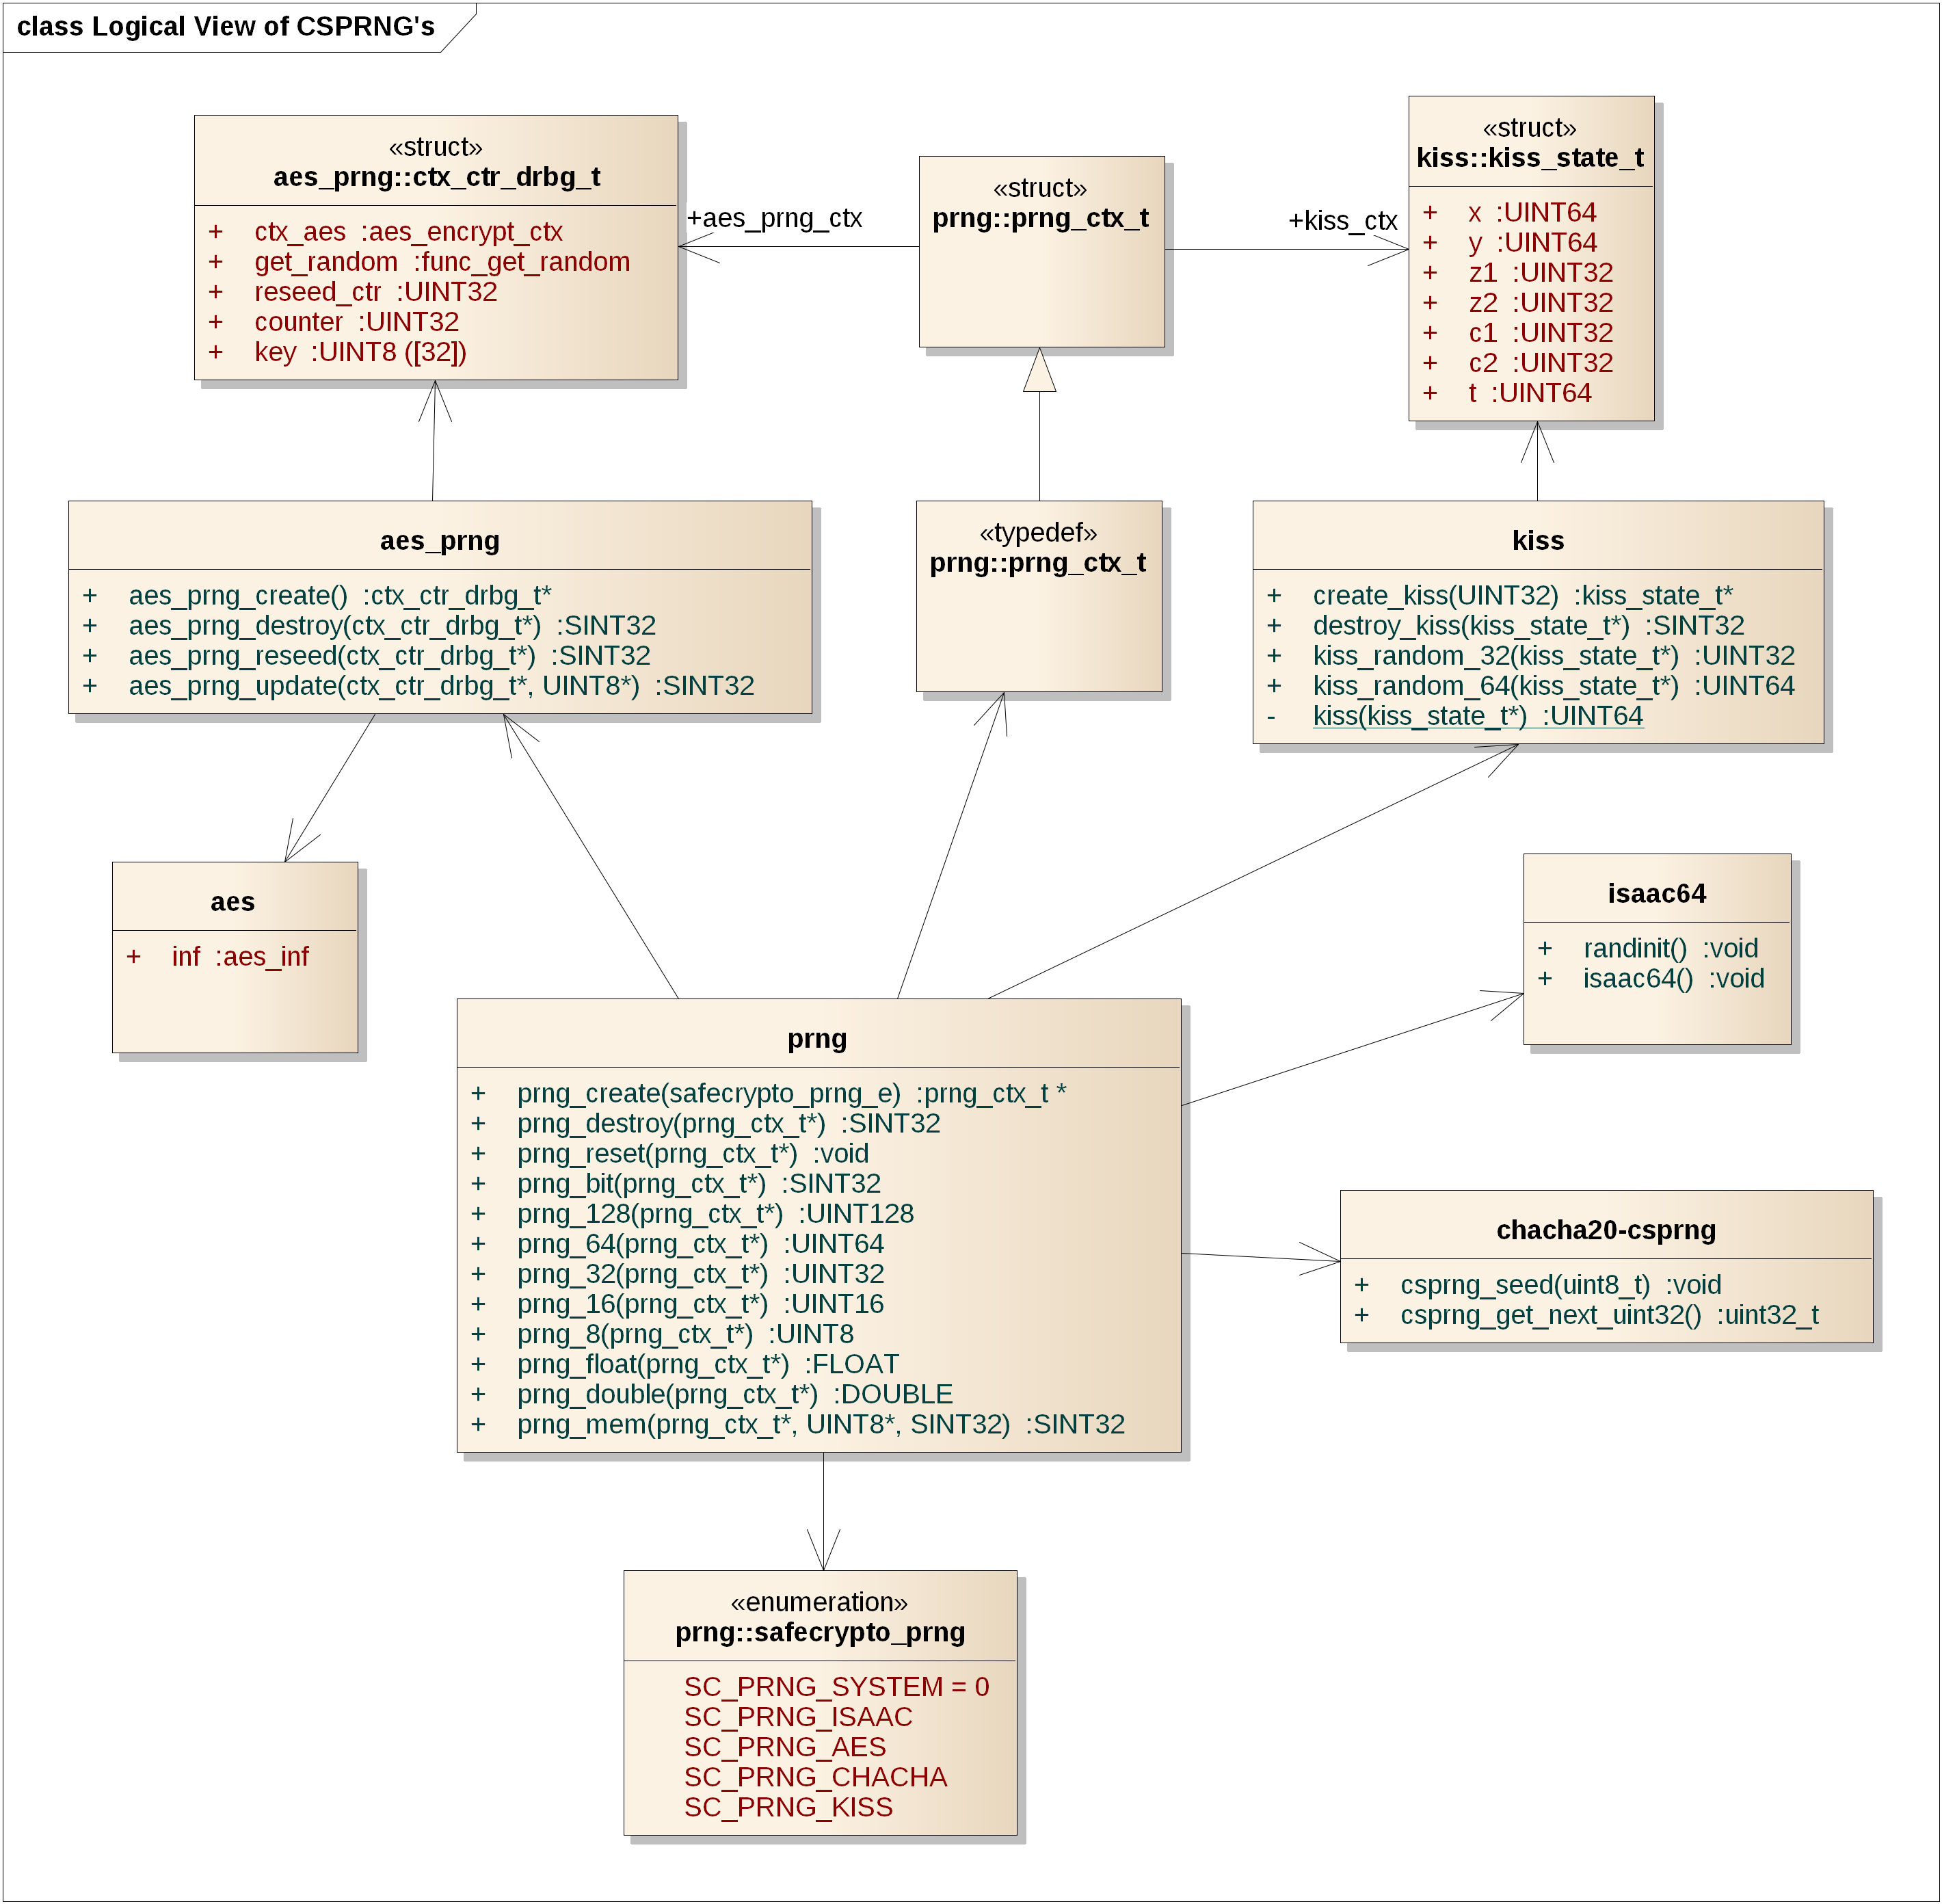
\includegraphics[width=\textwidth]{libsafecrypto_csprng_logical_view.png}
\caption{Class diagram of Cryptographically Secure PRNG's}
\label{fig:safecrypto_csprng}
\end{figure}


\newpage
\subsubsection{Gaussian Sampling}

All Gaussian Samplers implemented within the library will utilise the interface described in Figure \ref{fig:safecrypto_sampling}. A number of parameters common to all of the Samplers will be provided by a creation function, i.e. the required \textit{precision}, \textit{tailcut} and \textit{standard deviation}. The creation function will return a \textit{utils\_sampling\_t} struct containing the relevant function pointers and parameters for the selected Gaussian Sampler.

\begin{figure}[!h]
\centering
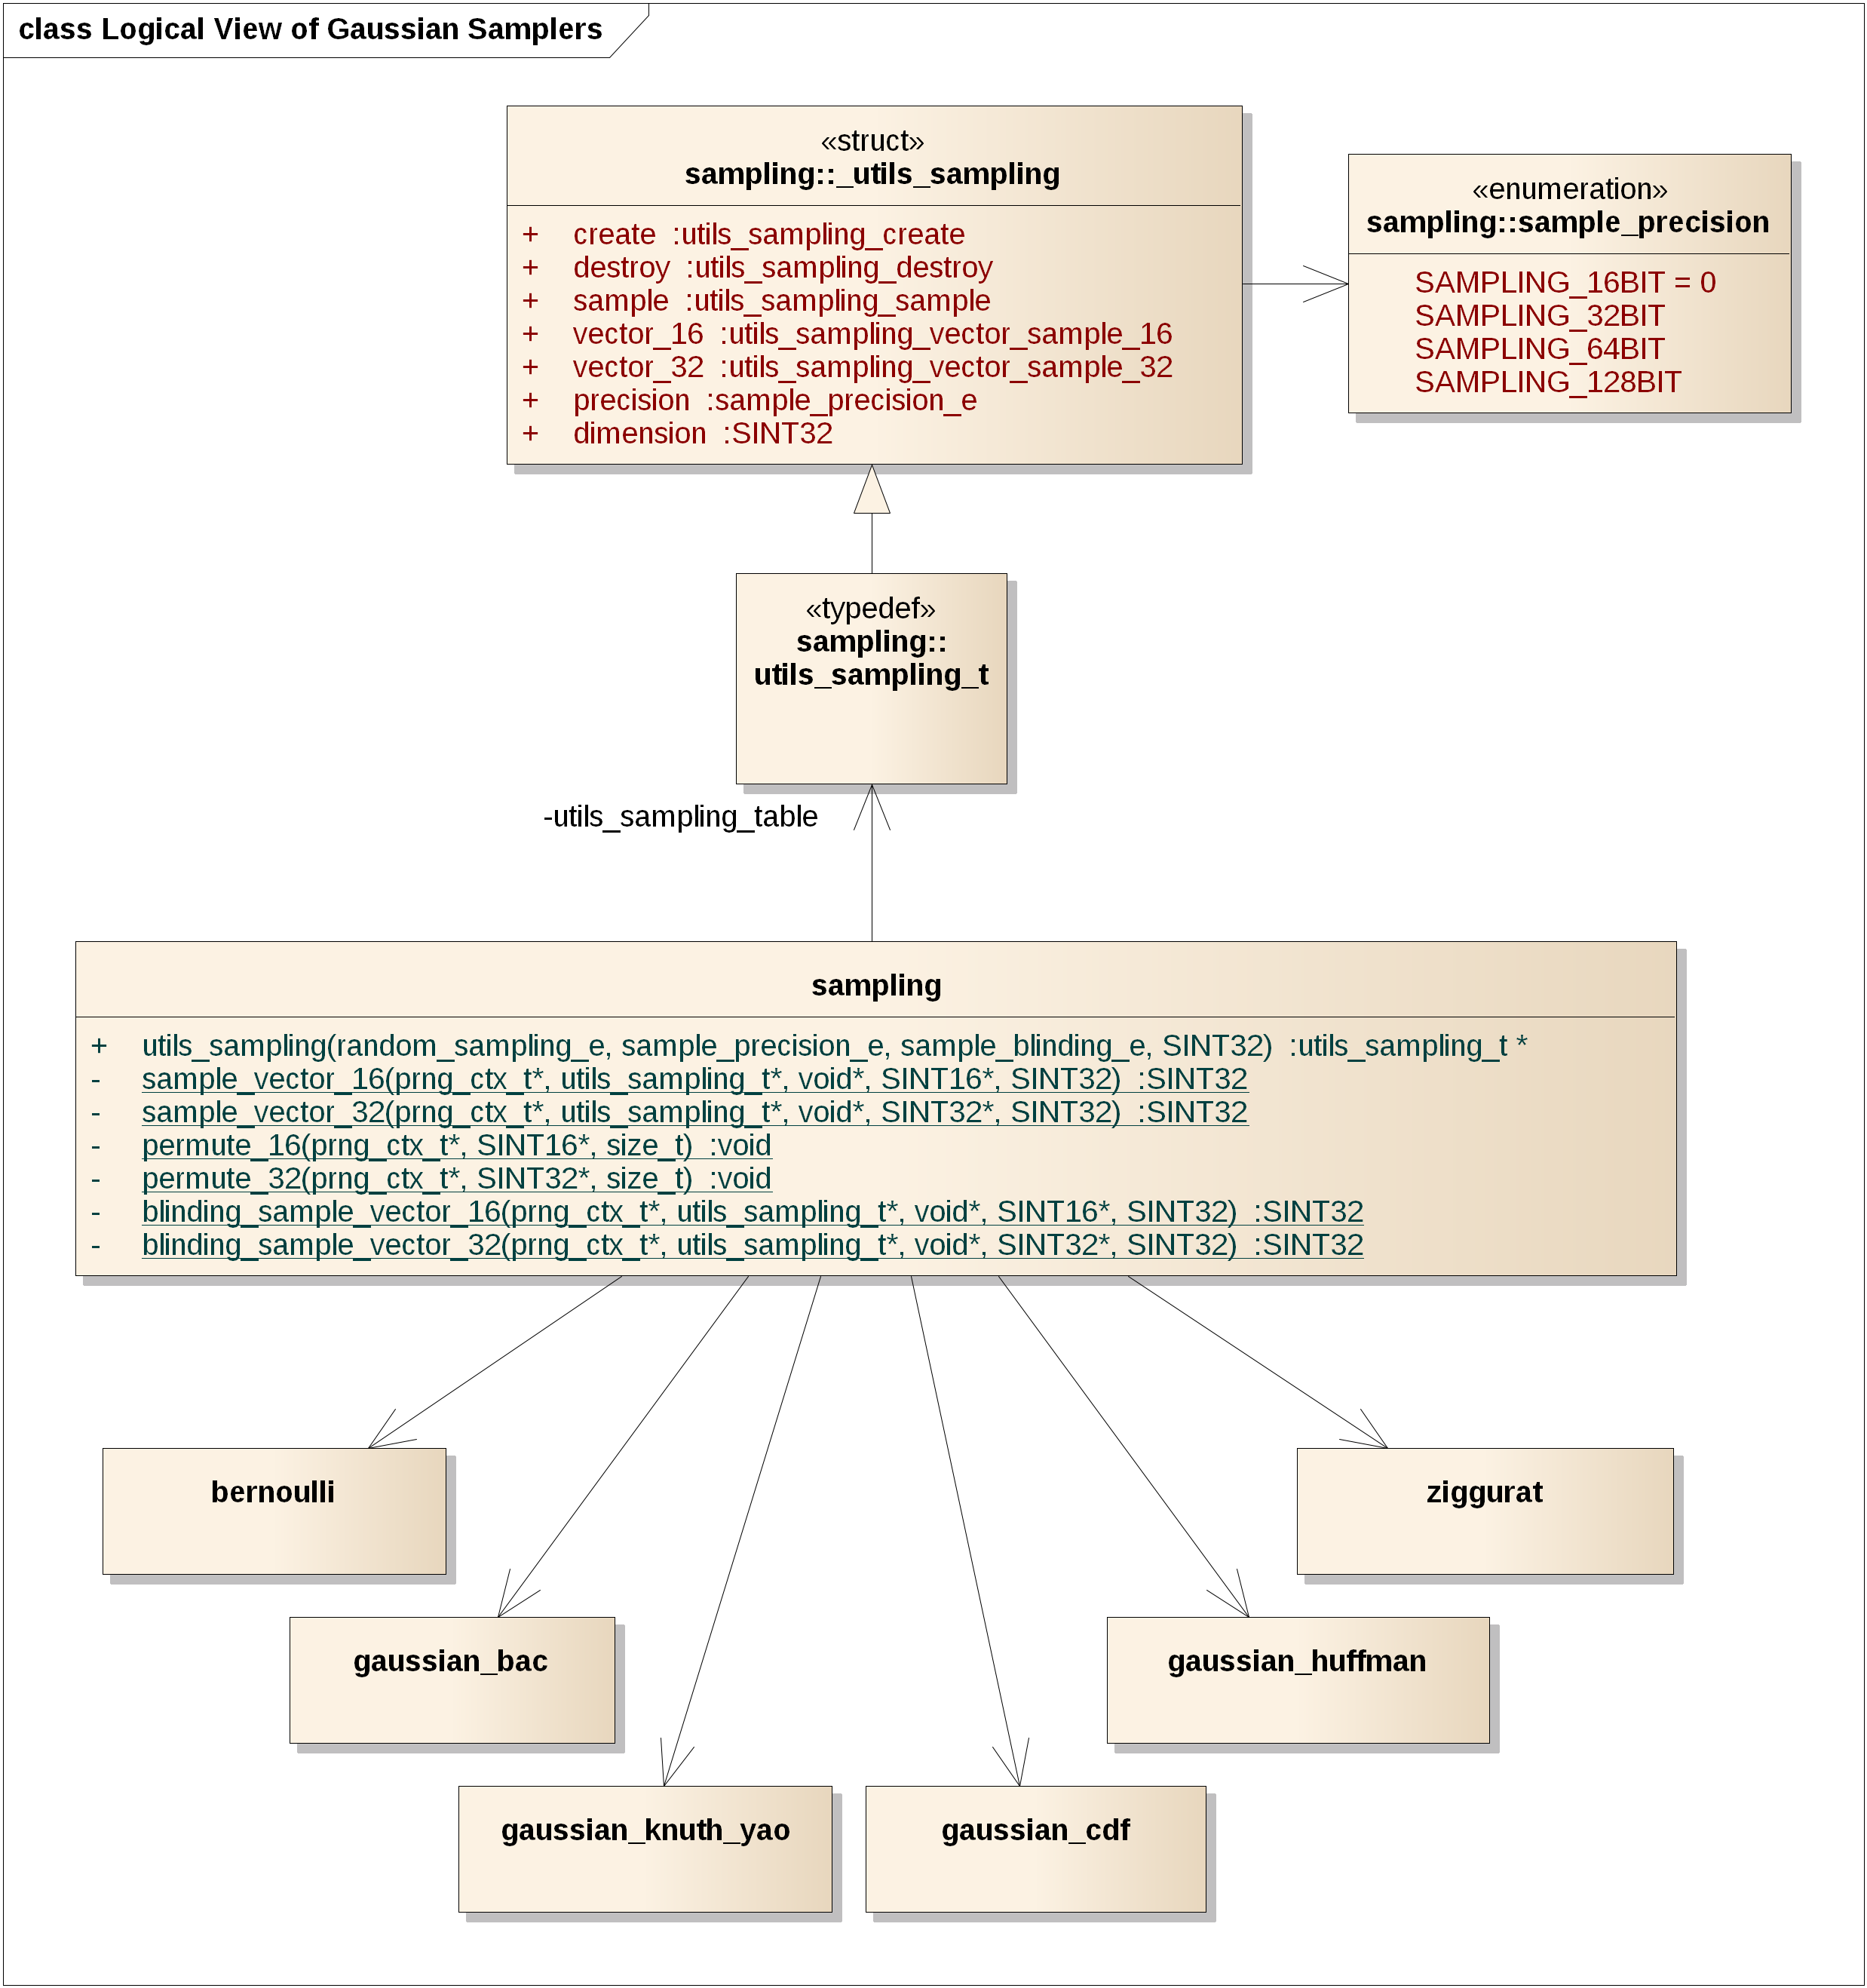
\includegraphics[width=\textwidth]{libsafecrypto_sampling_logical_view.png}
\caption{Class diagram of Gaussian Samplers}
\label{fig:safecrypto_sampling}
\end{figure}


\clearpage
\subsubsection{Entropy Coding}

The byte stream coding facility described in Figure \ref{fig:safecrypto_coding} will be used to provide all byte stream encoding and decoding with optional entropy coding. Lossless compression of keys and messages using a range of coding techniques will be provided by this convenience library. The interface permits compression to be dynamically configured.

\begin{figure}[!h]
\centering
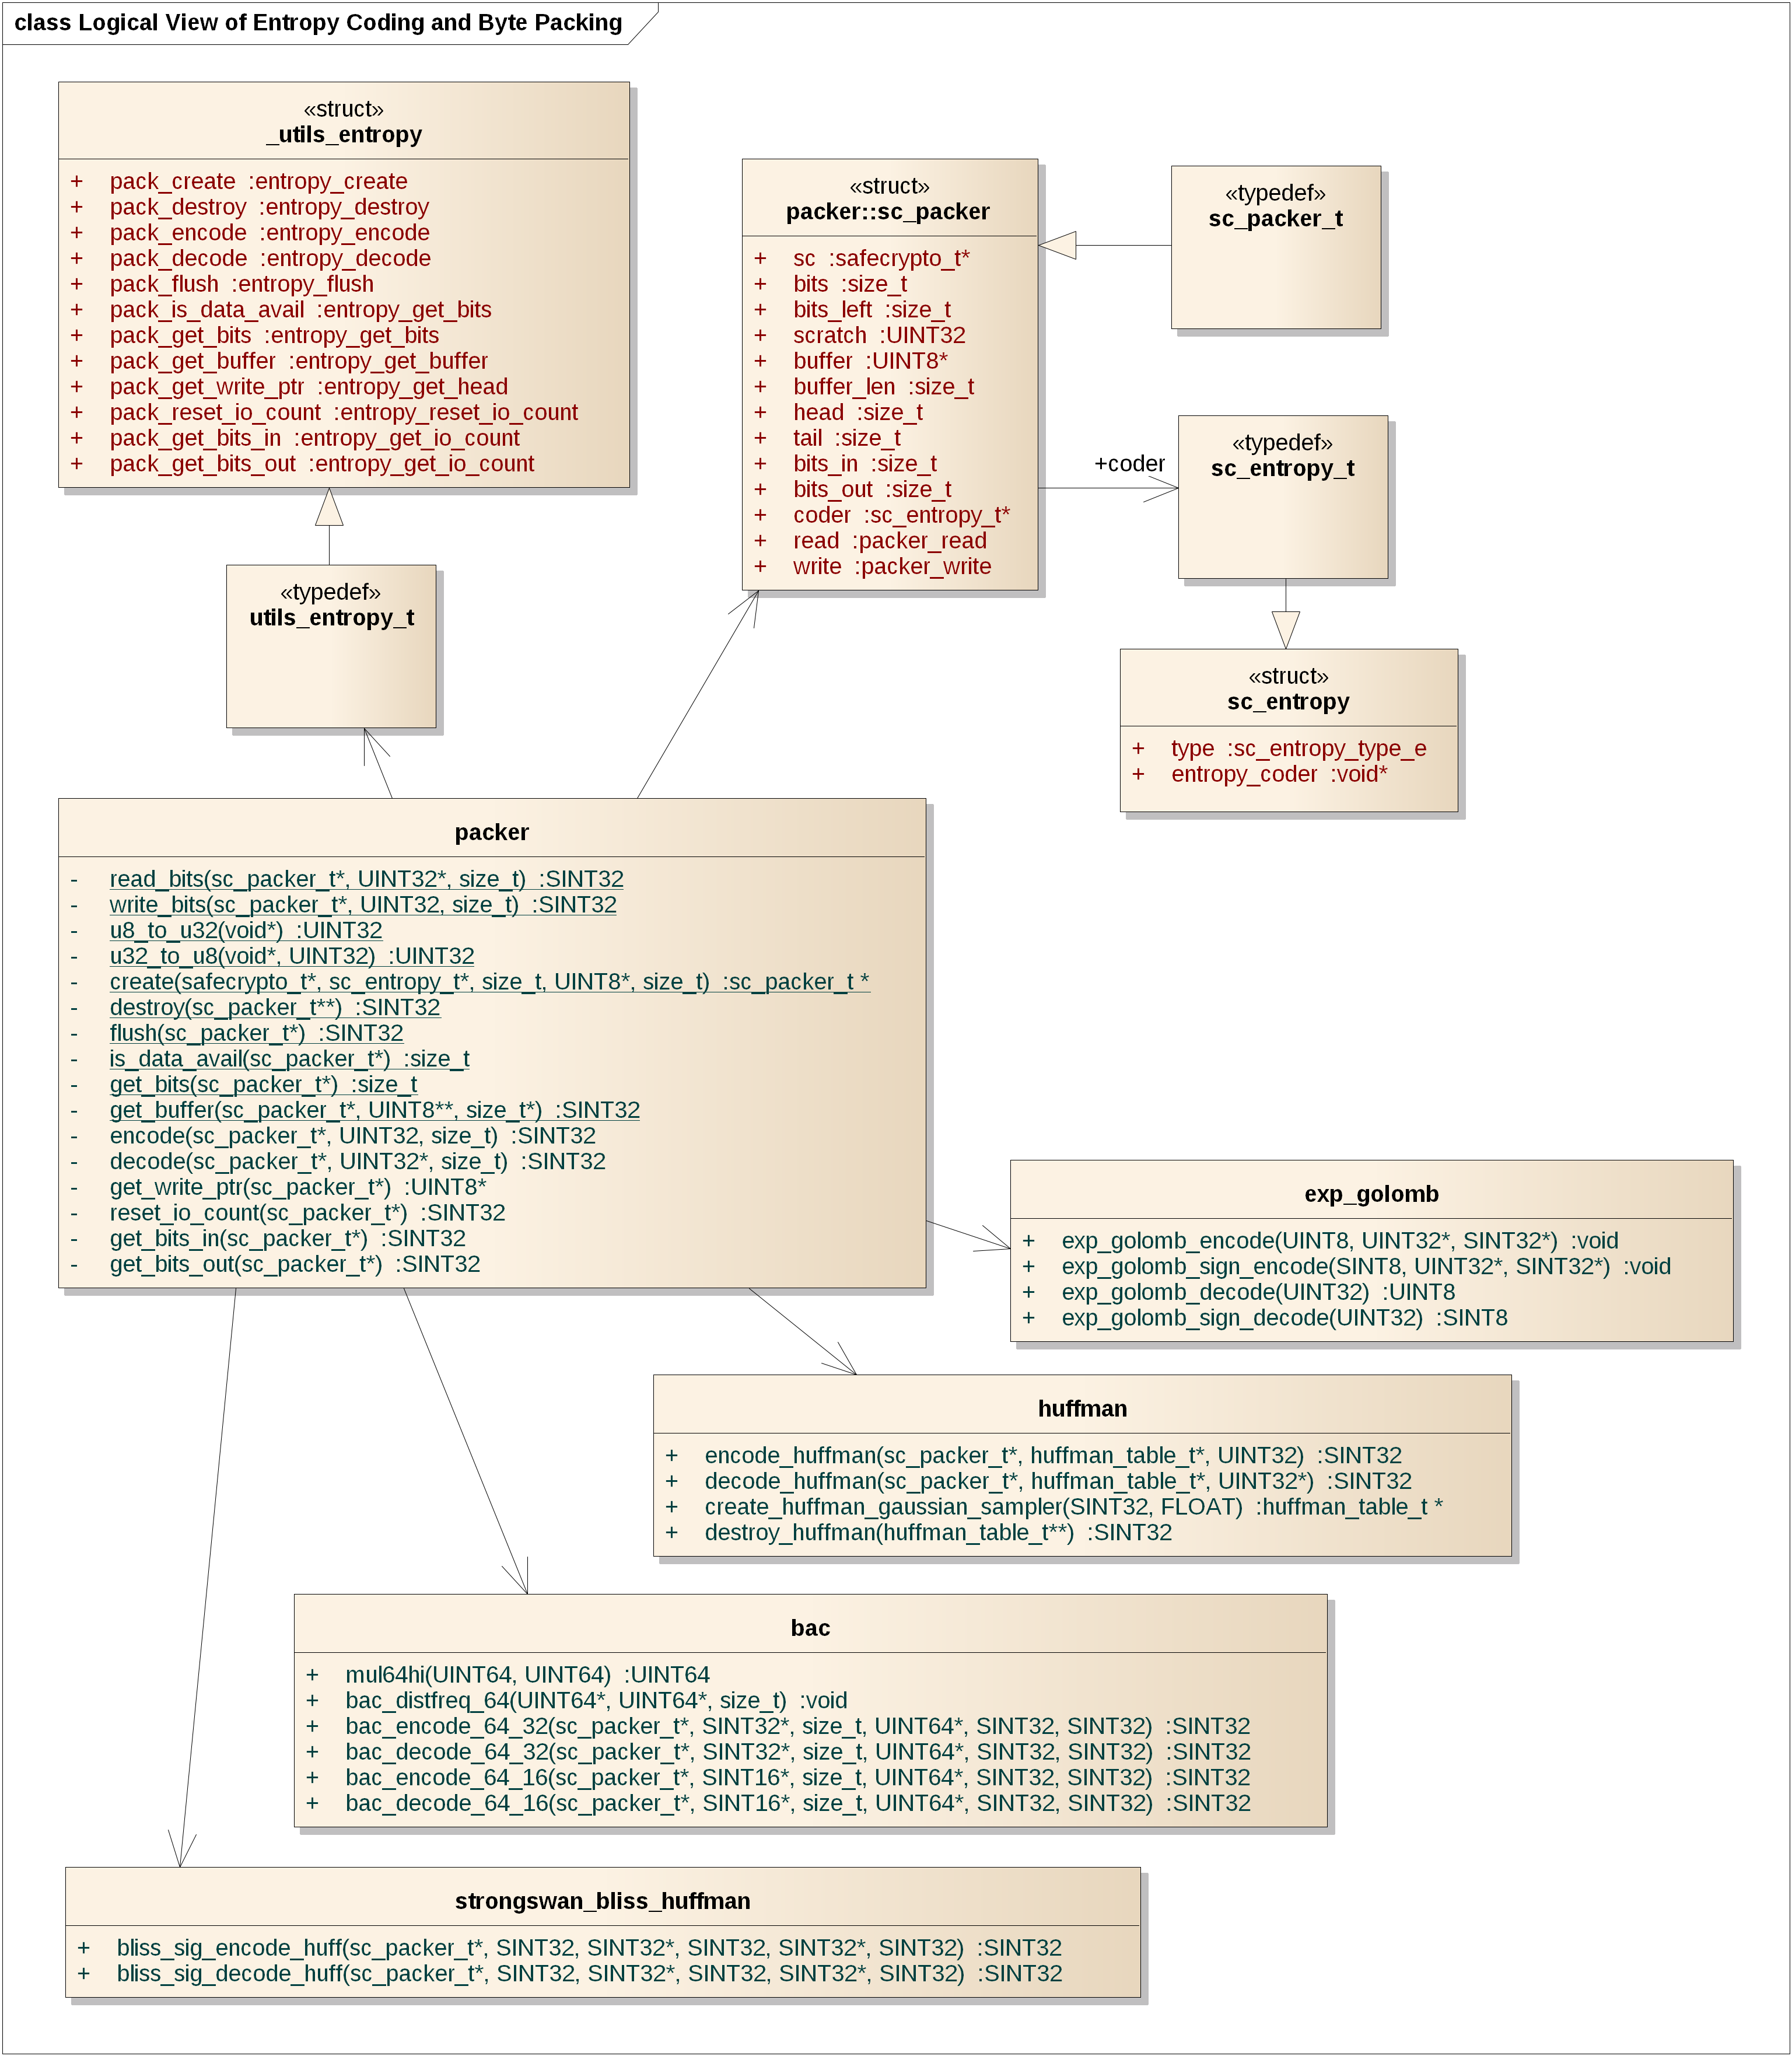
\includegraphics[width=\textwidth]{libsafecrypto_packer_logical_view.png}
\caption{Class diagram for byte stream coding}
\label{fig:safecrypto_coding}
\end{figure}

\newpage
The packer state is maintained by the struct \textit{sc\_packer\_t} thereby permitting multiple instances to be safely instantiated. It should be noted that of the three entropy coding schemes (Exponential Golomb coding, Binary Arithmetic Coding and Huffman Coding), Huffman coding is provided in two forms. The \textit{huffman} functions are associated with a generic implementation that can be readily applied to any scheme, but the \textit{strongswan\_bliss\_huffman} are associated with the Huffman codes used in the strongSwan BLISS implementation and are provided for comparative purposes.


\newpage
\subsubsection{Multithreading}

Multithreaded functionality will be provided for cross-platform operation. This will enable the SAFEcrypto library to provide guards and threading functions for those schemes that can exploit concurrency and/or parallelism. In addition to low-level functionality, high-level functions will be provided for threadpool and low-latency IPC.

The threading functionality is described in Figure \ref{fig:safecrypto_threading}. The \textit{threading} class provides all system-specific implementations of mutexes, threads, semaphores and condition variables. The implementations are hidden from the user using a common interface defined by the typedef'd struct \textit{utils\_threading\_t} that contains a list of function pointers that the user can call.

\begin{figure}[!h]
\centering
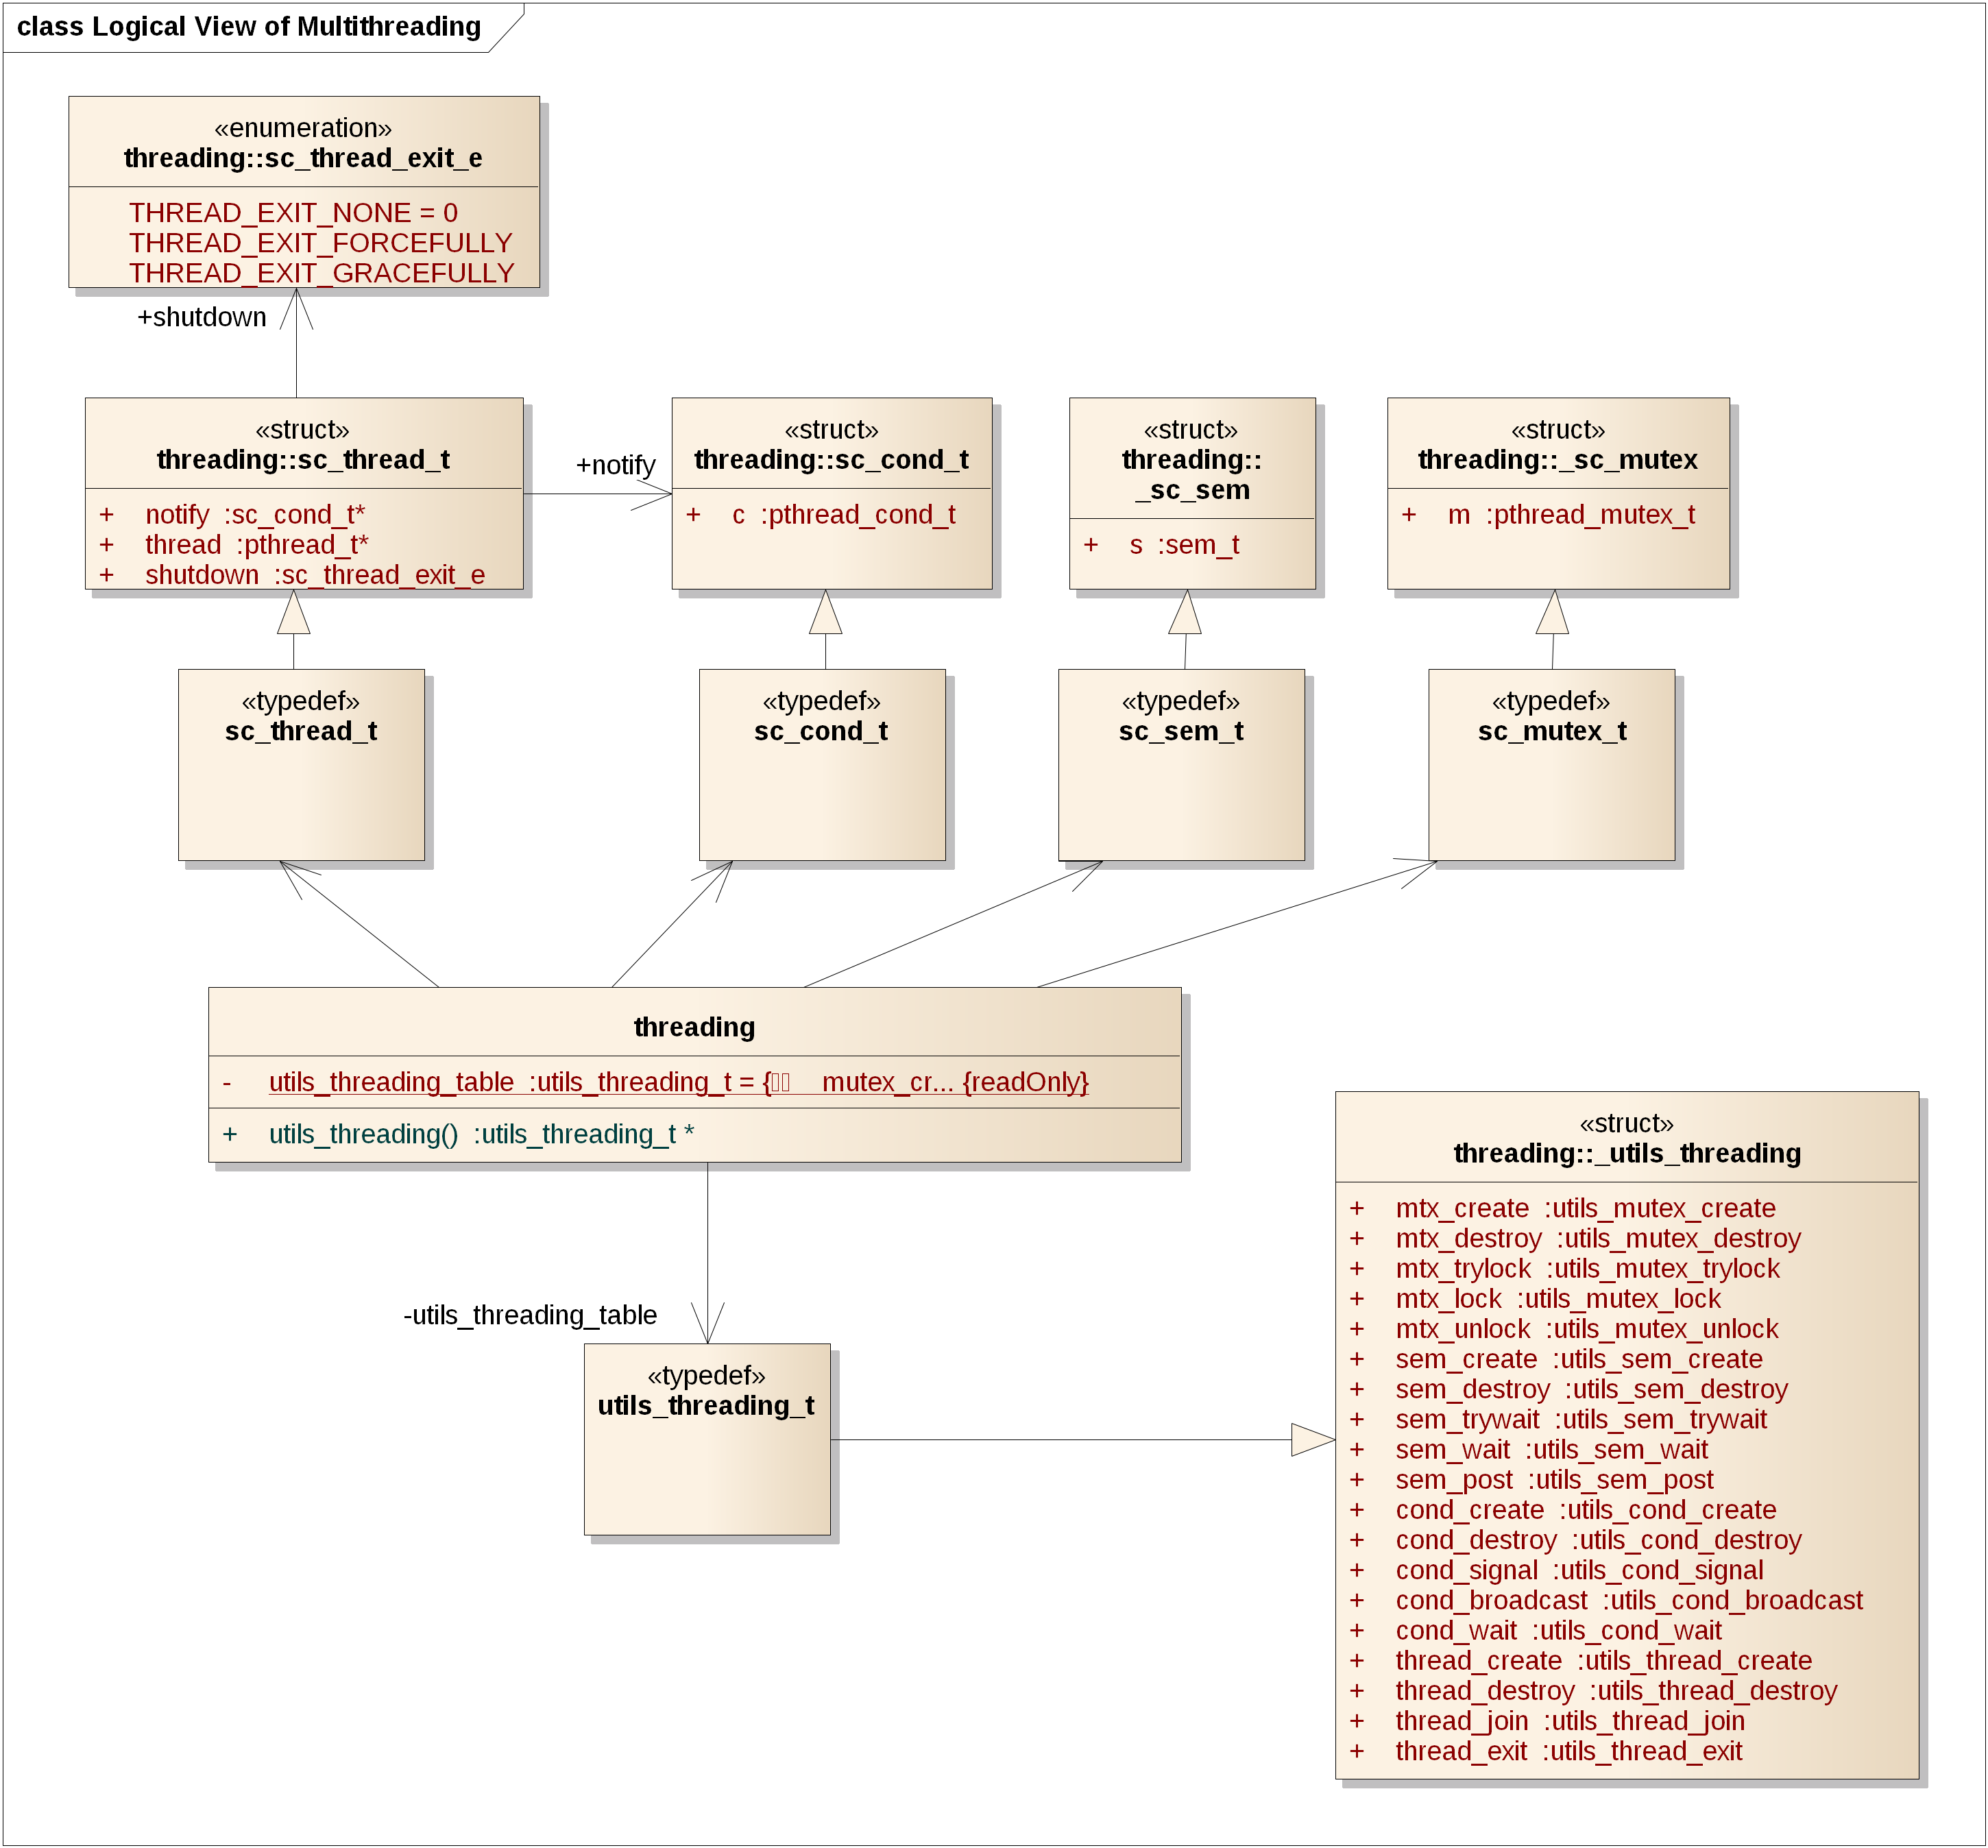
\includegraphics[width=\textwidth]{libsafecrypto_multithreading_logical_view.png}
\caption{Class diagram of multithreading capabilities}
\label{fig:safecrypto_threading}
\end{figure}

\newpage
The basic threading capabilities have been extended to provide a threadpool, as shown in Figure \ref{fig:safecrypto_threadpool}. The threadpool permits a number of worker threads to be instantiated and maintained in an idle state until. The user can supply tasks to be executed on the worker thread using a task queue. As tasks are queued the threadpool will notify the worker threads and supply the task using the \textit{sc\_threadpool\_task\_t} struct. When completed the threadpool will return the worker thread to a suspended state.

\begin{figure}[!h]
\centering
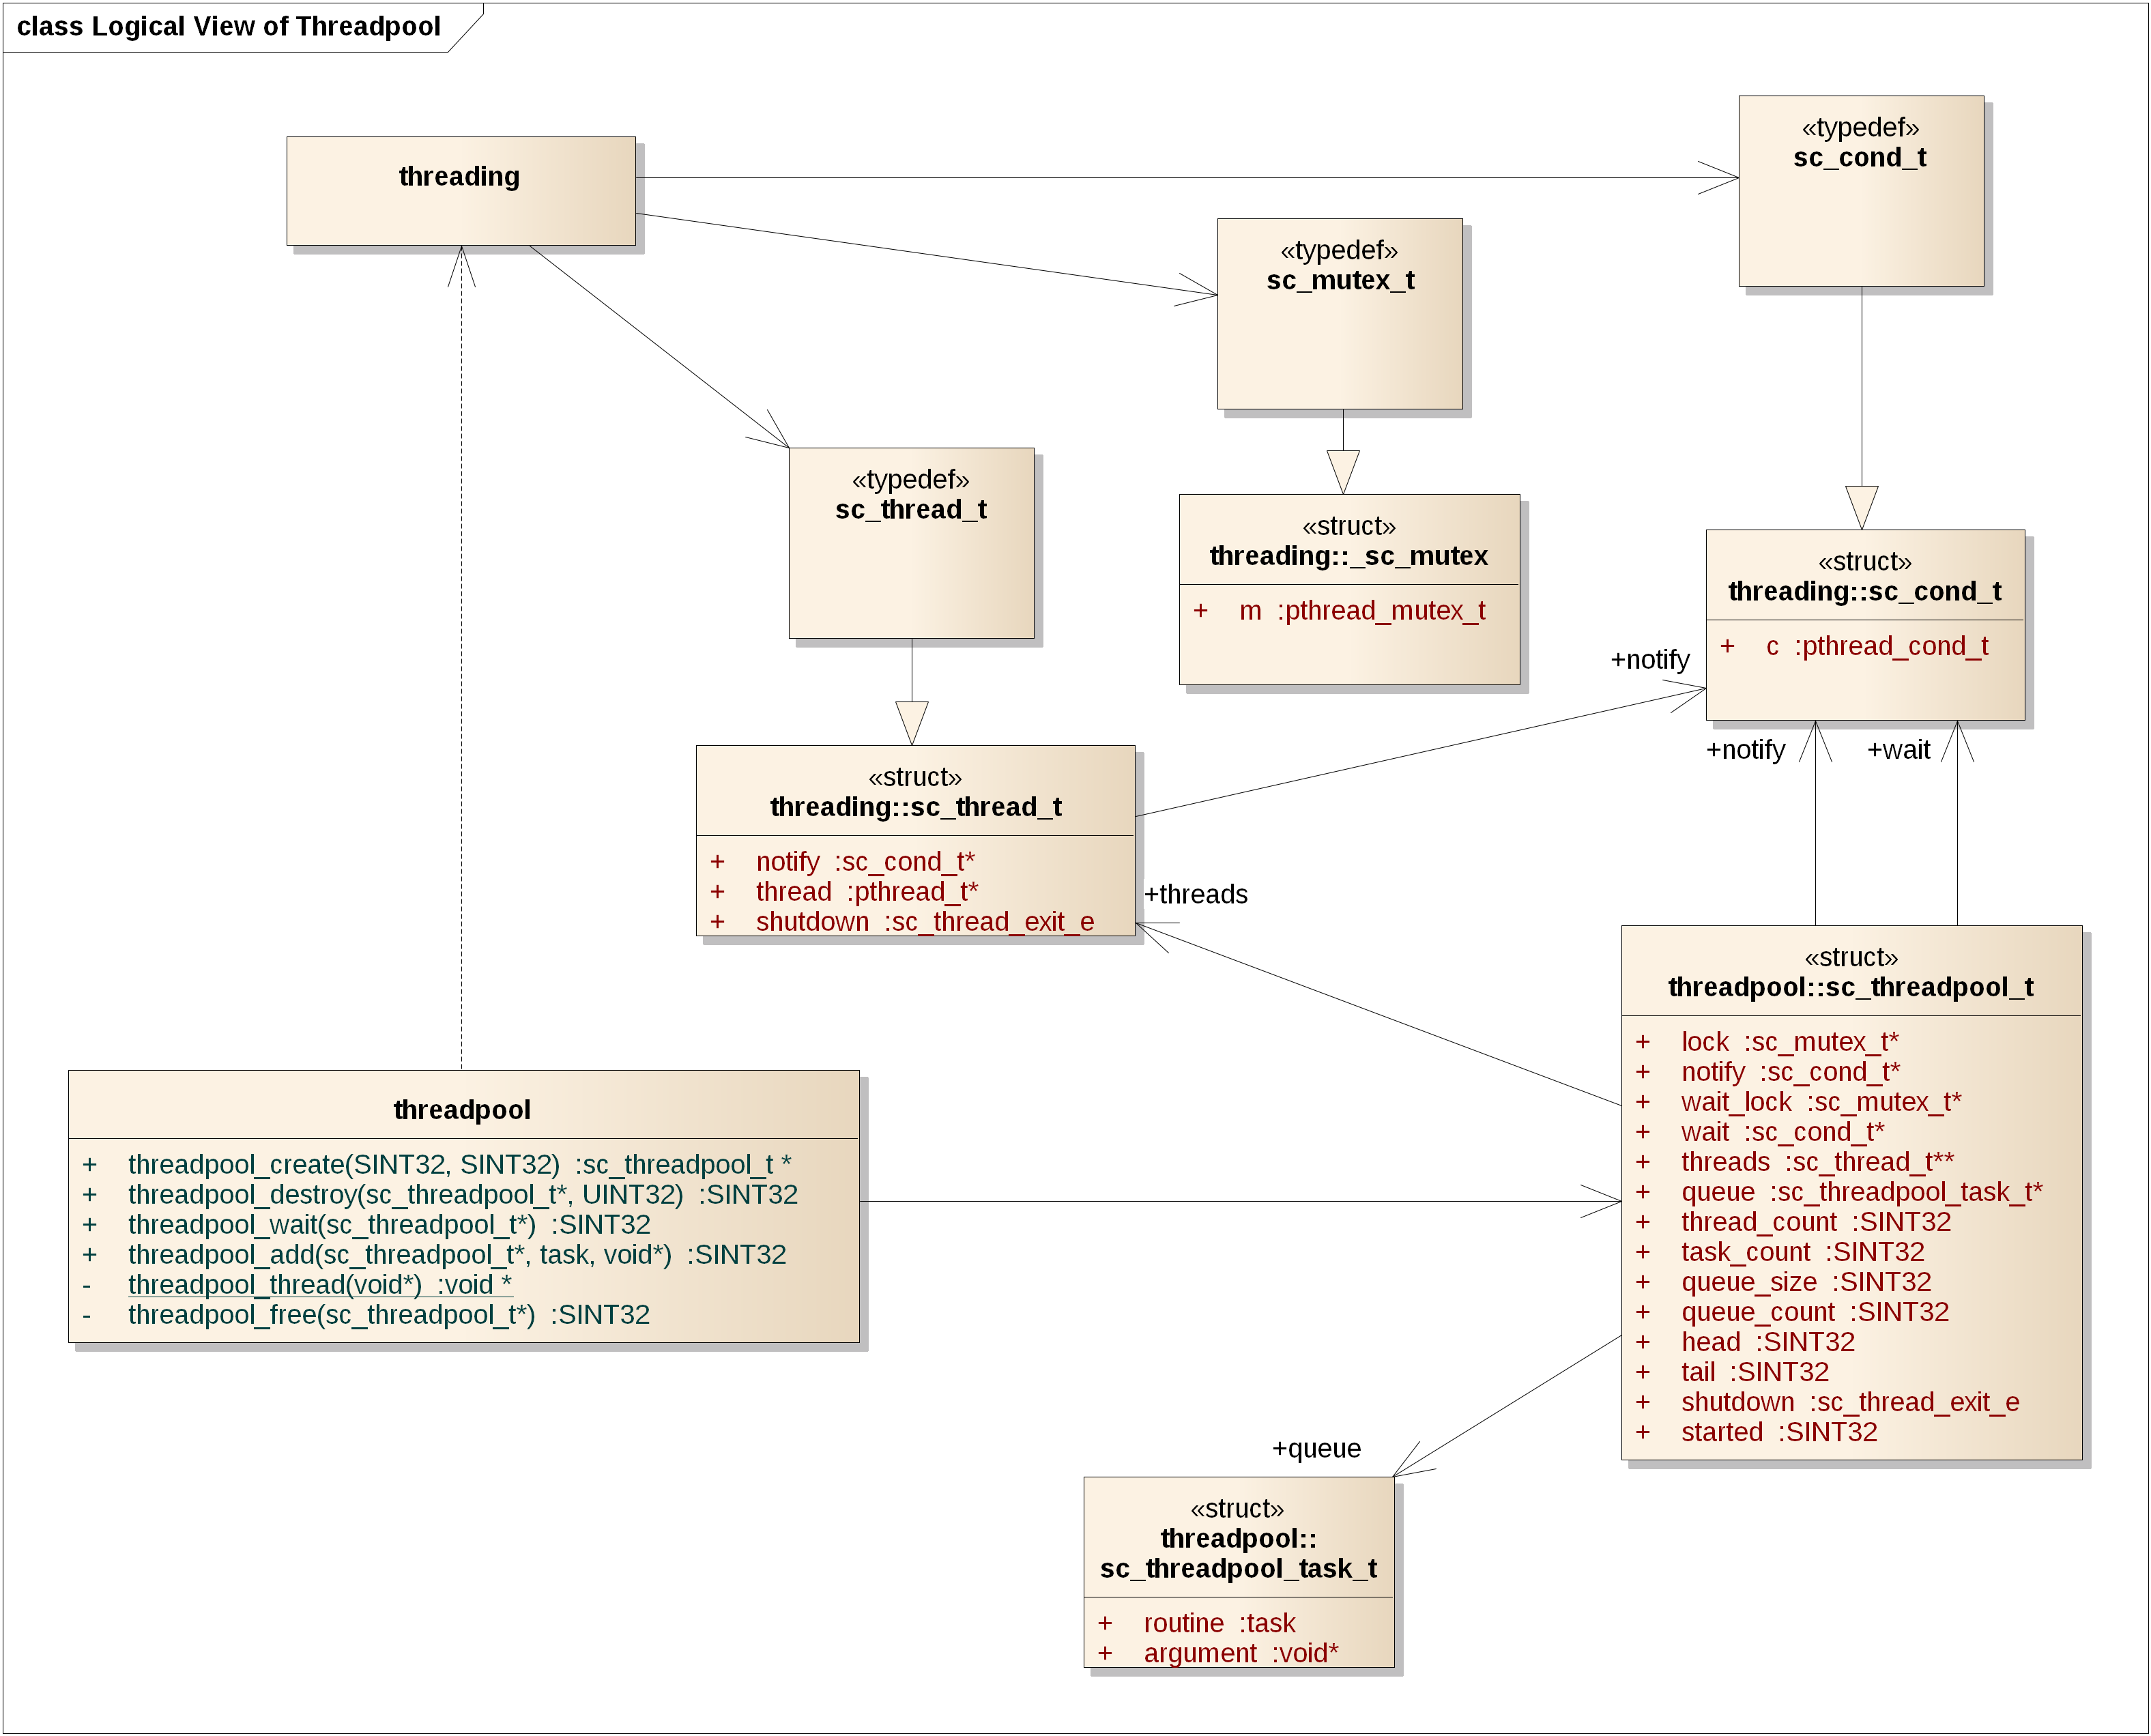
\includegraphics[width=\textwidth]{libsafecrypto_threadpool_logical_view.png}
\caption{Class diagram of threadpool}
\label{fig:safecrypto_threadpool}
\end{figure}

\newpage
Figure \ref{fig:safecrypto_pipe} provides a class diagram of the pipe inter-process communication (IPC) that is provided by the open-source project \textit{Pipe} by Clark Gaebel and ported into SAFEcrypto to use the SAFEcrypto library threading functionality described previously.

\begin{figure}[!h]
\centering
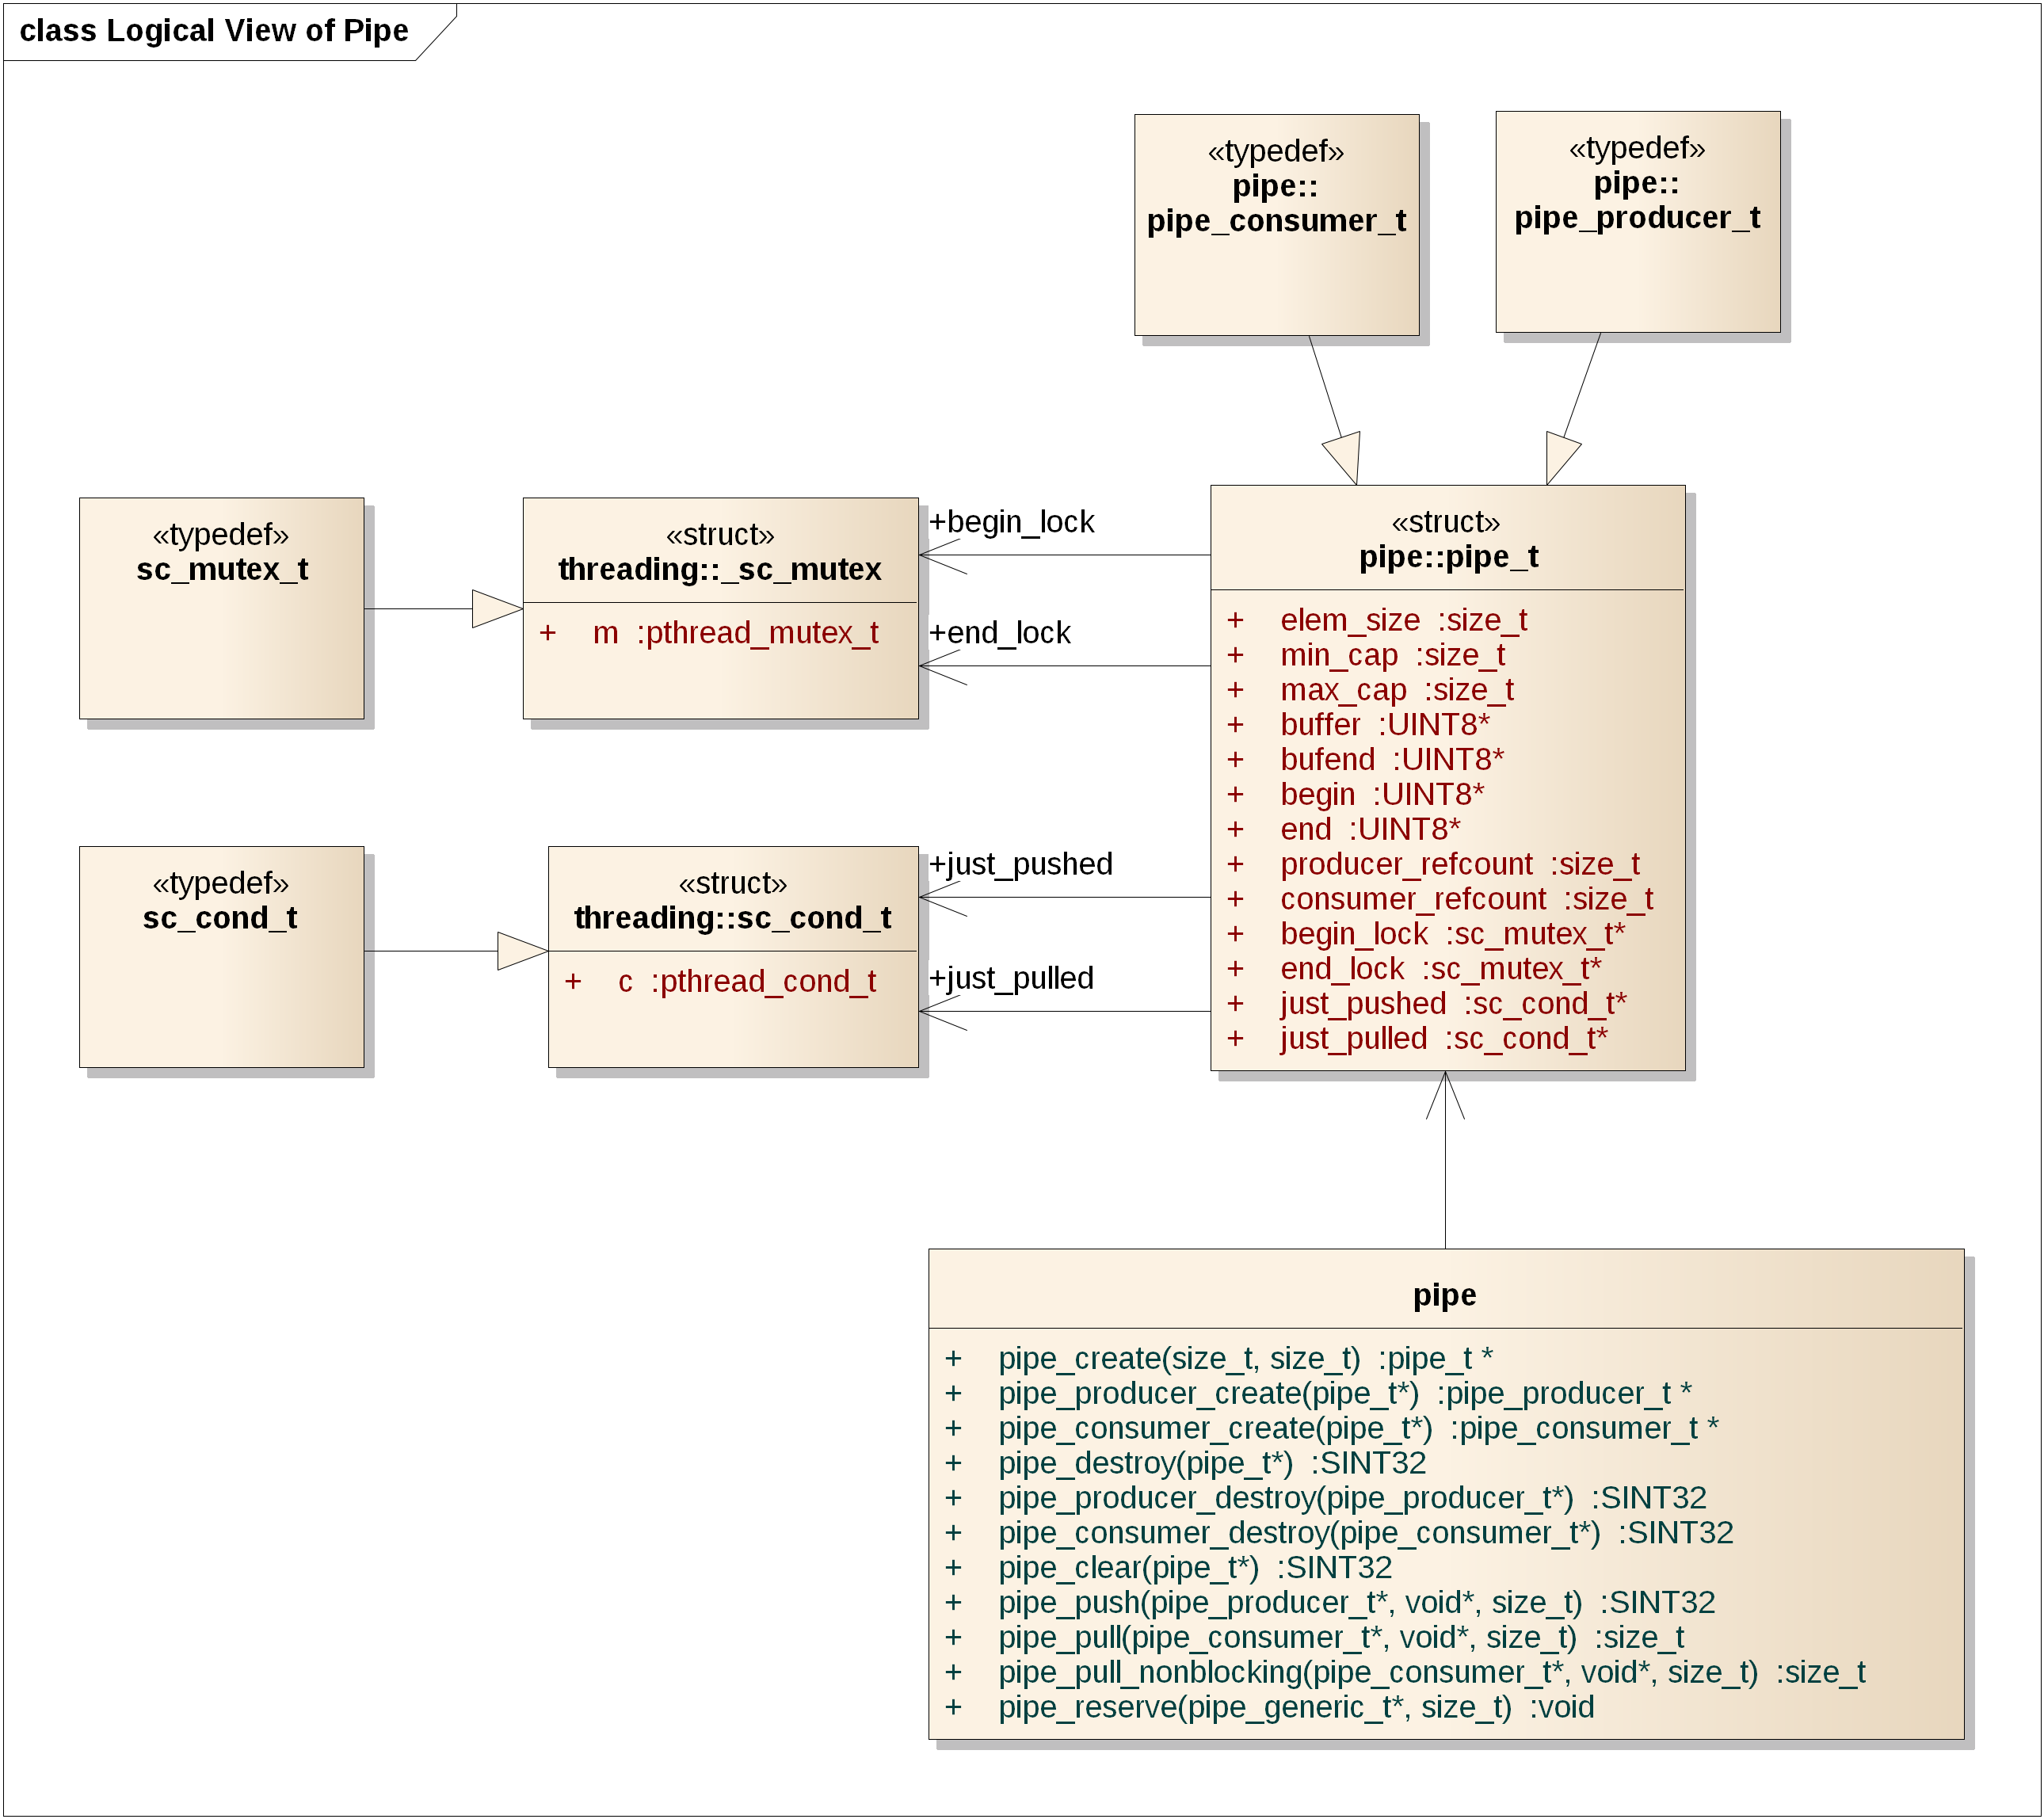
\includegraphics[width=\textwidth]{libsafecrypto_pipe_logical_view.png}
\caption{Class diagram of pipe IPC}
\label{fig:safecrypto_pipe}
\end{figure}

